\documentclass[compress,trans,9pt]{beamer}
% \documentclass[9pt]{beamer}
%\documentclass[compress,9pt,usenames,dvipsnames]{beamer}
% \usepackage[utf8]{inputenc}
% \includeonlyframes{current}
\setbeamercovered{dynamic}
\usepackage{etex}
\usepackage{graphicx,url,psfrag}
\usepackage{tikz}
\usetikzlibrary{
  decorations.pathreplacing,
  calc,
  decorations.fractals,
  through,
  shapes,
  patterns,
  arrows.meta,
  decorations.pathreplacing,
  arrows,
  shapes,
  mindmap
}
\usepackage[center]{subfigure}
\usepackage{enumerate}
\usepackage[makeroom]{cancel}
\usepackage{mathtools}
\usepackage{graphbox}
\usepackage{amssymb}
% \usepackage[showframe]{geometry}
% \usepackage{enumitem}

%
% for warning sign
%
\usepackage{stackengine}
\usepackage{scalerel}
\usepackage{xcolor}
\newcommand\dangersign[1][2ex]{%
  \renewcommand\stacktype{L}%
  \scaleto{\stackon[1.3pt]{\color{red}$\triangle$}{\tiny !}}{#1}%
}
% %  The following is to show codes:
\usepackage{listings}
% \usepackage{color}
\usepackage{colortbl}
\usepackage{dbt}

\definecolor{dkgreen}{rgb}{0,0.6,0}
\definecolor{gray}{rgb}{0.5,0.5,0.5}
\definecolor{mauve}{rgb}{0.58,0,0.82}

% \definecolor{deepblue}{rgb}{0,0,0.5}
% \definecolor{deepred}{rgb}{0.6,0,0}
% \definecolor{deepgreen}{rgb}{0,0.5,0}
% \lstset{
%   language=Python,
%   backgroundcolor=\color{red},  % choose the background color. You must add \usepackage{color}
%   % backgroundcolor=\color{background},  % choose the background color. You must add \usepackage{color}
%   basicstyle=\footnotesize,
%   otherkeywords={self},
%   keywordstyle=\ttb\color{deepblue},
%   emph={MyClass,__init__},
%   emphstyle=\ttb\color{deepred},
%   stringstyle=\color{deepgreen},
%   commentstyle=\color{red},  %%%%%%%%
%   frame=tb,
%   showstringspaces=false
% }
%
% \lstdefinestyle{Python}{
%     language        = Python,
%     basicstyle      = \footnotesize,
%     keywordstyle    = \color{blue},
%     keywordstyle    = [2] \color{red}, % just to check that it works
%     stringstyle     = \color{green},
%     commentstyle    = \color{red}\ttfamily
% }

\lstset{frame=tb,
  language=Java,
  aboveskip=3mm,
  belowskip=3mm,
  showstringspaces=false,
  columns=flexible,
  basicstyle={\small\ttfamily},
  numbers=none,
  numberstyle=\tiny\color{gray},
  keywordstyle=\color{blue},
  commentstyle=\color{dkgreen},
  stringstyle=\color{mauve},
  breaklines=true,
  breakatwhitespace=true,
  tabsize=3
}
\lstset{language=Java}

\lstset{ %
  language=R,                     % the language of the code
  basicstyle=\footnotesize,       % the size of the fonts that are used for the code
  numbers=left,                   % where to put the line-numbers
  numberstyle=\tiny\color{gray},  % the style that is used for the line-numbers
  stepnumber=1,                   % the step between two line-numbers. If it's 1, each line
                                  % will be numbered
  numbersep=5pt,                  % how far the line-numbers are from the code
  backgroundcolor=\color{background},  % choose the background color. You must add \usepackage{color}
  showspaces=false,               % show spaces adding particular underscores
  showstringspaces=false,         % underline spaces within strings
  showtabs=false,                 % show tabs within strings adding particular underscores
  frame=single,                   % adds a frame around the code
  rulecolor=\color{black},        % if not set, the frame-color may be changed on line-breaks within not-black text (e.g. commens (green here))
  tabsize=2,                      % sets default tabsize to 2 spaces
  captionpos=b,                   % sets the caption-position to bottom
  breaklines=true,                % sets automatic line breaking
  breakatwhitespace=false,        % sets if automatic breaks should only happen at whitespace
  title=\lstname,                 % show the filename of files included with \lstinputlisting;
                                  % also try caption instead of title
  keywordstyle=\color{blue},      % keyword style
  commentstyle=\color{dkgreen},   % comment style
  stringstyle=\color{mauve},      % string literal style
  escapeinside={\%*}{*)},         % if you want to add a comment within your code
  morekeywords={*,...}            % if you want to add more keywords to the set
}
% \usepackage[usenames,dvipsnames]{color}
% \lstset{
%   language=Python,                     % the language of the code
%   basicstyle=\footnotesize,       % the size of the fonts that are used for the code
%   numbers=left,                   % where to put the line-numbers
%   numberstyle=\tiny\color{gray},  % the style that is used for the line-numbers
%   stepnumber=1,                   % the step between two line-numbers. If it's 1, each line
%                                   % will be numbered
%   numbersep=5pt,                  % how far the line-numbers are from the code
%   backgroundcolor=\color{background},  % choose the background color. You must add \usepackage{color}
%   showspaces=false,               % show spaces adding particular underscores
%   showstringspaces=false,         % underline spaces within strings
%   showtabs=false,                 % show tabs within strings adding particular underscores
%   frame=single,                   % adds a frame around the code
%   rulecolor=\color{black},        % if not set, the frame-color may be changed on line-breaks within not-black text (e.g. commens (green here))
%   tabsize=2,                      % sets default tabsize to 2 spaces
%   captionpos=b,                   % sets the caption-position to bottom
%   breaklines=true,                % sets automatic line breaking
%   breakatwhitespace=false,        % sets if automatic breaks should only happen at whitespace
%   title=\lstname,                 % show the filename of files included with \lstinputlisting;
%                                   % also try caption instead of title
%   keywordstyle=\ttb\color{blue},      % keyword style
%   commentstyle=\color{dkgreen},   % comment style
%   stringstyle=\color{mauve},      % string literal style
%   escapeinside={\%*}{*)},         % if you want to add a comment within your code
%   morekeywords={*,...}            % if you want to add more keywords to the set
% }

% \usepackage[dvipsnames]{xcolor}
% \newcommand{\Cross}{\mathbin{\tikz [x=1.4ex,y=1.4ex,line width=.2ex] \draw (0,0) -- (1,1) (0,1) -- (1,0);}}%
\newcommand{\Crossme}[1]{\!\!
\tikz [black,x=1.1em,y=1.1em,line width=.4ex]
\draw (-0.5,-0.5) -- (0,0) node {\footnotesize #1} -- (0.5,0.5) (0.5,-0.5) -- (-0.5,0.5);}%
\newcommand{\Checkme}[1]{\!\!
\tikz [x=1.1em,y=1.1em,line width=.4ex]
\draw [black] (0,0.7) -- (0.3,0) --(0.9,1.0) (0.5,0.5) node {\footnotesize #1};}
% \beamerdefaultoverlayspecification{<+-| alert@+>} %(this will show line by line)
\beamerdefaultoverlayspecification{<+->} %(this will show line by

% \usepackage{natbib}
% \input{../myMathSymbols.tex}
% \newcommand{\tlMr}[4]{\:{}^{\hspace{0.2em}#1}_{#2} \hspace{-0.1em}#3_{#4}}

% Smiley face\Smiley{} \Frowny{}
\usepackage{marvosym}
% -------------------------------------------------
%  Set directory for figs
% -------------------------------------------------
\usepackage{grffile}
\graphicspath{{Codes/}}
% -------------------------------------------------
%  Define colors
% -------------------------------------------------
\def\refcolor{cyan}
\newcommand{\myref}[1]{\small {\em #1}}
\def\excolor{brown}
% \usepackage{color}
% \usepackage[dvipsnames]{xcolor}


% % % Define danger sign
\newcommand*{\TakeFourierOrnament}[1]{{%
\fontencoding{U}\fontfamily{futs}\selectfont\char#1}}
\newcommand*{\danger}{\TakeFourierOrnament{66}}


% -------------------------------------------------
%  Define short-hand symbols.
% -------------------------------------------------
\newcommand{\B}{\textbf{B}}
\newcommand{\PP}{\mathbb{P}}
\newcommand{\E}{\mathbb{E}}
\newcommand{\D}{\mathbb{D}}
\newcommand{\W}{\dot{W}}
\newcommand{\ud}{\ensuremath{\mathrm{d}}}
\newcommand{\Ceil}[1]{\left\lceil #1 \right\rceil}
\newcommand{\Floor}[1]{\left\lfloor #1 \right\rfloor}
\newcommand{\sgn}{\text{sgn}}
\newcommand{\Lad}{\text{L}_{\text{ad}}^2}
\newcommand{\SI}[1]{\mathcal{I}\left[#1 \right]}
\newcommand{\SIB}[2]{\mathcal{I}_{#2}\left[#1 \right]}
\newcommand{\Indt}[1]{1_{\left\{#1 \right\}}}
\newcommand{\LadInPrd}[1]{\left\langle #1 \right\rangle_{\text{L}_\text{ad}^2}}
\newcommand{\LadNorm}[1]{\left|\left|  #1 \right|\right|_{\text{L}_\text{ad}^2}}
\newcommand{\Norm}[1]{\left|\left|  #1   \right|\right|}
\newcommand{\Ito}{It\^{o} }
\newcommand{\Itos}{It\^{o}'s }
\newcommand{\spt}[1]{\text{supp}\left(#1\right)}
\newcommand{\InPrd}[1]{\left\langle #1 \right\rangle}
\newcommand{\mr}{\textbf{r}}
\newcommand{\Ei}{\text{Ei}}
\newcommand{\arctanh}{\operatorname{arctanh}}
\newcommand{\ind}[1]{\mathbb{I}_{\left\{ {#1} \right\} }}
\newcommand{\Var}{\text{Var}}
\newcommand{\Cov}{\text{Cov}}
\newcommand{\Corr}{\text{Corr}}

\newcommand{\baseurl}[1]{\footnotesize\url{http://math.emory.edu/~lchen41/teaching/2020_Spring/#1}}


\newcommand*\mystrut[1]{\vrule width0pt height0pt depth#1\relax} % adding vertical space

\DeclareMathOperator{\esssup}{\ensuremath{ess\,sup}}

\newcommand{\steps}[1]{\vskip 0.3cm \textbf{#1}}
\newcommand{\calB}{\mathcal{B}}
\newcommand{\calC}{\mathcal{C}}
\newcommand{\calD}{\mathcal{D}}
\newcommand{\calE}{\mathcal{E}}
\newcommand{\calF}{\mathcal{F}}
\newcommand{\calG}{\mathcal{G}}
\newcommand{\calK}{\mathcal{K}}
\newcommand{\calH}{\mathcal{H}}
\newcommand{\calI}{\mathcal{I}}
\newcommand{\calL}{\mathcal{L}}
\newcommand{\calM}{\mathcal{M}}
\newcommand{\calN}{\mathcal{N}}
\newcommand{\calO}{\mathcal{O}}
\newcommand{\calT}{\mathcal{T}}
\newcommand{\calP}{\mathcal{P}}
\newcommand{\calR}{\mathcal{R}}
\newcommand{\calS}{\mathcal{S}}
\newcommand{\calV}{\mathcal{V}}
\newcommand{\bbC}{\mathbb{C}}
\newcommand{\bbN}{\mathbb{N}}
\newcommand{\bbP}{\mathbb{P}}
\newcommand{\bbZ}{\mathbb{Z}}
\newcommand{\myVec}[1]{\overrightarrow{#1}}
\newcommand{\sincos}{\begin{array}{c} \cos \\ \sin \end{array}\!\!}
\newcommand{\CvBc}[1]{\left\{\:#1\:\right\}}
\newcommand*{\one}{{{\rm 1\mkern-1.5mu}\!{\rm I}}}

\newcommand{\OneFrame}[1]{
\begin{enumerate}\item[#1] \phantom{av} \\[20em]\vfill\phantom{av}\myEnd\end{enumerate}}

\newcommand{\bH}{\ensuremath{\mathrm{H}}}
\newcommand{\Ai}{\ensuremath{\mathrm{Ai}}}

\newcommand{\R}{\mathbb{R}}
\newcommand{\myEnd}{\hfill$\square$}
\newcommand{\myQED}{\hfill\textcolor{lgtblue}{$\blacksquare$}}
\newcommand{\ds}{\displaystyle}
\newcommand{\Shi}{\text{Shi}}
\newcommand{\Chi}{\text{Chi}}
\newcommand{\Erf}{\ensuremath{\mathrm{erf}}}
\newcommand{\Erfc}{\ensuremath{\mathrm{erfc}}}
\newcommand{\He}{\ensuremath{\mathrm{He}}}
\newcommand{\Res}{\ensuremath{\mathrm{Res}}}

\newcommand{\mySeparateLine}{\begin{center}
 \makebox[\linewidth]{\rule{0.6\paperwidth}{0.4pt}}
\end{center}}

\theoremstyle{definition}
% \newtheorem{definition}[theorem]{Definition}
% \newtheorem{hypothesis}[theorem]{Hypothesis}
\newtheorem{assumption}[theorem]{Assumption}

\theoremstyle{plain}
% \newtheorem{theorem}{Theorem}
% \newtheorem{corollary}[theorem]{Corollary}
% \newtheorem{lemma}[theorem]{Lemma}
\newtheorem{proposition}[theorem]{Proposition}

\mode<presentation>
{
%      \usetheme{Warsaw}
%     \usetheme{JuanLesPins}
%  \usetheme{Hannover}
%  \usetheme{Montpellier}
   \useoutertheme{default}
  % or ...

  \setbeamercovered{transparent}
  % or whatever (possibly just delete it)
 \setbeamertemplate{frametitle}{
  \begin{centering}
    \color{blue}
    {\insertframetitle}
    \par
  \end{centering}
  }
}
\usefoottemplate{\hfill \insertframenumber{}}
% \inserttotalframenumber

\usepackage[english]{babel}
% or whatever

% \usepackage[latin1]{inputenc}
% or whatever

\usepackage{times}
\usepackage[T1]{fontenc}
% Or whatever. Note that the encoding and the font should match. If T1
% does not look nice, try deleting the line with the fontenc.

% \DeclareMathOperator{\Lip}{Lip}
\DeclareMathOperator{\lip}{l}
% \DeclareMathOperator{\Vip}{\overline{v}}
% \DeclareMathOperator{\vip}{\underline{v}}
% \DeclareMathOperator{\vv}{v}
% \DeclareMathOperator{\BC}{BC}
% \DeclareMathOperator{\CH}{CD}

\usepackage{pgfpages}
% \setbeameroption{show notes}
% \setbeamertemplate{note page}[plain]
% \setbeameroption{second mode text on second screen=right}
% \setbeameroption{show notes on second screen=right}
%
\title % (optional, use only with long paper titles)
{
Math 362: Mathematical Statistics II
}

% \subtitle
% {Research Plan} % (optional)

\author{Le Chen\\
\url{le.chen@emory.edu}\\
\url{chenle02@gmail.com}\\[2em]
Emory University\\
Atlanta, GA\\[2em]
\textcolor{gray}{\small Last updated on Spring 2021}\\
\textcolor{gray}{\small Last compiled on \today}
}
\institute[Emory University]
{%
\vspace{3em}
% \pgfuseimage{UNLV}
 }
 \vfill
% - Use the \inst command only if there are several affiliations.
% - Keep it simple, no one is interested in your street address.

% \date[Talk at Karlsruhe] % (optional)
% {\today }
 \date[Columbus]{
   2021 Spring\\[1em]
   Creative Commons License\\
   (CC By-NC-SA)
 }

\subject{}
% This is only inserted into the PDF information catalog. Can be left
% out.

% If you have a file called "university-logo-filename.xxx", where xxx
% is a graphic format that can be processed by latex or pdflatex,
% resp., then you can add a logo as follows:

% \pgfdeclareimage[height=0.8cm]{UNLV}{figs/UNLV-186.png}

% Delete this, if you do not want the table of contents to pop up at
% the beginning of each subsection:
% \AtBeginSubsection[]
% {
%   \begin{frame}<beamer>{Outline}
%     \tableofcontents[currentsection,currentsubsection]
%   \end{frame}
% }


% If you wish to uncover everything in a step-wise fashion, uncomment
% the following command:

% \beamerdefaultoverlayspecification{<+->}
% % % % % % % % % % % % % % % % % % %
%  Define a block
% % % % % % % % % % % % % % % % % % %
\newenvironment<>{problock}[1]{%
  \begin{actionenv}#2%
      \def\insertblocktitle{#1}%
      \par%
      \mode<presentation>{%
        \setbeamercolor{block title}{fg=white,bg=olive!95!black}
       \setbeamercolor{block body}{fg=black,bg=olive!25!white}
       \setbeamercolor{itemize item}{fg=white!20!white}
       \setbeamertemplate{itemize item}[triangle]
     }%
      \usebeamertemplate{block begin}}
    {\par\usebeamertemplate{block end}\end{actionenv}}

\newenvironment<>{assblock}[1]{%
  \begin{actionenv}#2%
      \def\insertblocktitle{#1}%
      \par%
      \mode<presentation>{%
        \setbeamercolor{block title}{fg=white,bg=green!50!black}
       \setbeamercolor{block body}{fg=black,bg=green!10}
       \setbeamercolor{itemize item}{fg=green!80!black}
       \setbeamertemplate{itemize item}[triangle]
     }%
      \usebeamertemplate{block begin}}
    {\par\usebeamertemplate{block end}\end{actionenv}}


\newcommand{\mySection}[1]{\section{\S\: #1}\begin{frame}{\myChapter}\tableofcontents[currentsection]\end{frame}}

\AtBeginSection[]
  {
     \begin{frame}<beamer>
     \frametitle{Plan}
     \tableofcontents[currentsection]
     \end{frame}
  }


\begin{document}

\AtBeginSection[]
  {
     \begin{frame}<beamer>
     \frametitle{Plan}
     \tableofcontents[currentsection]
     \end{frame}
  }


%-------------- start slide -------------------------------%{{{
\begin{frame}[noframenumbering]
  \titlepage
\end{frame}
%-------------- end slide -------------------------------%}}}


% \begin{frame}{Outline}
%   \tableofcontents
%   % You might wish to add the option [pausesections]
% \end{frame}

\newcommand{\myChapter}{Chapter 7. Inference Based on The Normal Distribution}

%-------------- start slide -------------------------------%{{{
\begin{frame}
\begin{center}
\huge
\myChapter
\end{center}
\end{frame}
%-------------- end slide -------------------------------%}}}
\mySection{7.1 Introduction}
%-------------- start slide -------------------------------%{{{ 7.4.
\begin{frame}
% {\S\: 7.1 Introduction}
	\centering
		\begin{minipage}{0.4\textwidth}
\centering
		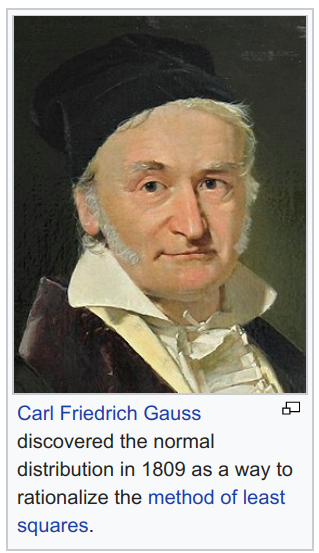
\includegraphics[scale=0.25]{Gauss.png}
		(1777-1855)
\end{minipage}
		\qquad
		\begin{minipage}{0.4\textwidth}
\centering
		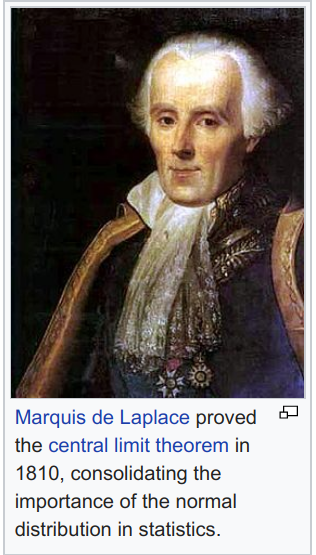
\includegraphics[scale=0.25]{Laplace.png}
		(1749-1827)
\end{minipage}
\end{frame}
%-------------- end slide -------------------------------%}}}
%-------------- start slide -------------------------------%{{{ 7.5.
\begin{frame}
	\centering
	\begin{minipage}{0.28\textwidth}
		\centering
	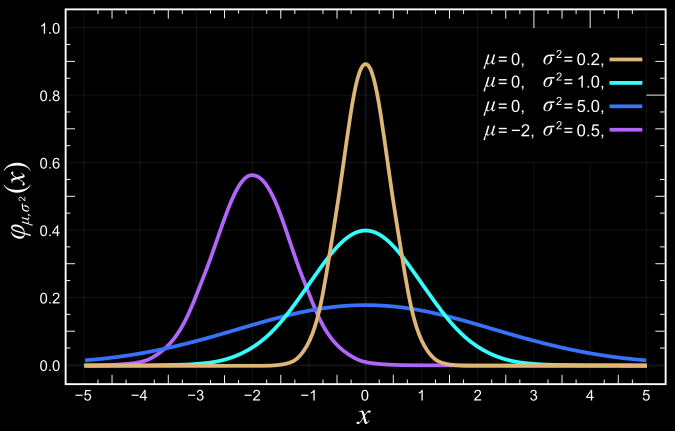
\includegraphics[scale=0.23]{Normal_Distribution_PDF-neg.png}
\end{minipage}
% \hspace{3em}
\hfill
\begin{minipage}{0.63\textwidth}
	\centering
	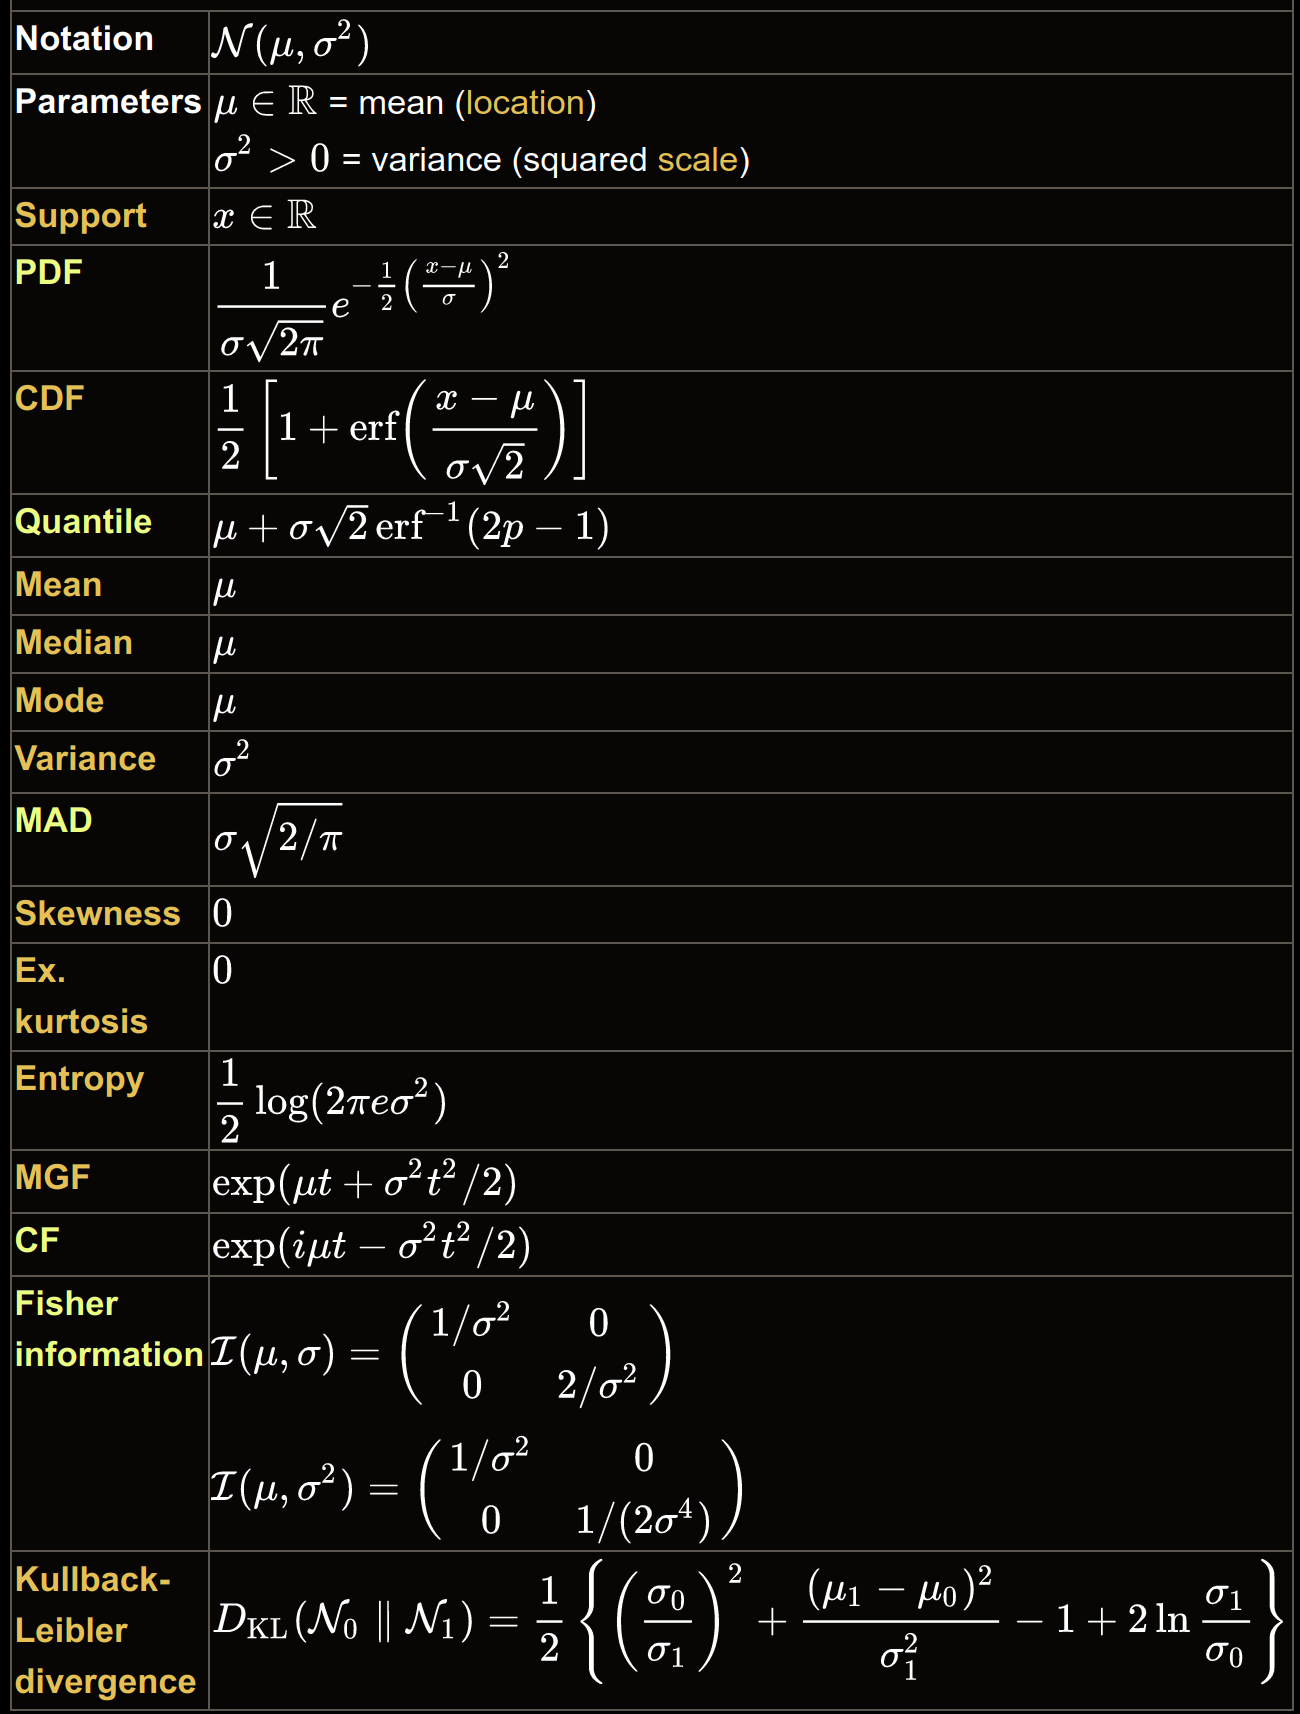
\includegraphics[scale=0.13]{Normal_List_Properties-neg.png}
\end{minipage}
\vfill
\footnotesize
\url{https://en.wikipedia.org/wiki/Normal_distribution}
\end{frame}
%-------------- end slide -------------------------------%}}}
%-------------- start slide -------------------------------%{{{ 7.6.
\begin{frame}{Test for normal parameters (one sample test)}
\begin{enumerate}
	\item[Let] $Y_1,\cdots,Y_n$ be a random sample from $N(\mu,\sigma^2)$.
		\vfill
	\item[Prob. 1] Find a test statistic $\Lambda$ in order to test\hfill $H_0 : \mu = \mu_0$ v.s. $H_1 : \mu \ne \mu_0$. \\[2em]
	\item[]When $\sigma^2$ is known: \hspace{4em}
		$\displaystyle	\Lambda =  \frac{\overline{Y}-\mu_0}{\sigma/\sqrt{n}}\sim N(0,1)$\\[1em]
\item[] When $\sigma^2$ is unknown: \hspace{3em} $\displaystyle \Lambda = \alert{?}$
	\pause \hspace{3em}
	$\displaystyle	\Lambda \stackrel{\alert{?}}{=}  \frac{\overline{Y}-\mu_0}{s/\sqrt{n}}\quad \sim\quad \alert{?}$
	\vfill
	\item[Prob. 2] Find a test statistic $\Lambda$ in order to test\hfill $H_0 : \sigma^2 = \sigma_0^2$ v.s. $H_1 : \sigma^2 \ne \sigma^2_0$. \\[2em]
\end{enumerate}
\end{frame}
%-------------- end slide -------------------------------%}}}
%-------------- start slide -------------------------------%{{{ 7.7.
\begin{frame}
	\begin{enumerate}
	\item[Prob. 1] Find a test statistic for $H_0 : \mu = \mu_0$ v.s. $H_1 : \mu \ne \mu_0$, with $\sigma^2$ unknown\\[2em]
		\vfill
\item[Sol.] Composite-vs-composite test with:
\[\omega =\left\{(\mu,\sigma^2): \mu=\mu_0, \: \sigma^2>0\right\}\]
\[\Omega =\left\{(\mu,\sigma^2): \mu\in\R, \: \sigma^2>0\right\}\]\\[2em]
\item[] The MLE under the two spaces are:
	\begin{align}\tag{Under $\omega$}
		\omega_e=(\mu_e,\sigma_e^2): \qquad
		\mu_e =\mu_0	\quad\text{and}\quad \sigma_e^2 = \frac 1n \sum_{i=1}^n (y_i-\mu_0)^2
	\end{align}
	\begin{align}\tag{Under $\Omega$}
		\Omega_e=(\mu_e,\sigma_e^2): \qquad
		\mu_e =\bar{y}	\quad\text{and}\quad \sigma_e^2 = \frac 1n \sum_{i=1}^n (y_i-\bar{y})^2
	\end{align}
	\end{enumerate}
\end{frame}
%-------------- end slide -------------------------------%}}}
%-------------- start slide -------------------------------%{{{ 7.8.
\begin{frame}
	\begin{enumerate}
		\item[]
			\[
				L(\mu,\sigma^2) = (2\pi \sigma^2)^{-n} \exp \left( -\frac{1}{2} \sum_{i=1}^n \left(  \frac{y_i-\mu}{\sigma} \right)^2\right)
			\]
			\vfill
		\item[]	\[
				L(\omega_e) =  \cdots  = \left[  \frac{ne^{-1}}{2\pi\sum_{i=1}^n (y_i-\mu_0)^2}\right]^{n/2}
			\]
			\bigskip
			\[
				L(\Omega_e) =  \cdots  = \left[  \frac{ne^{-1}}{2\pi\sum_{i=1}^n (y_i-\bar{y})^2}\right]^{n/2}
			\]
		\end{enumerate}
\end{frame}
%-------------- end slide -------------------------------%}}}
%-------------- start slide -------------------------------%{{{ 7.9.
\begin{frame}

\begin{enumerate}
		\item[] Hence,
		\begin{align*}
			\lambda = \frac{L(\omega_e)}{L(\Omega_e)} & = \left[  \frac{\sum_{i=1}^n (y_i-\bar{y})^2}{\sum_{i=1}^n (y_i-\mu_0)^2}\right]^{n/2} = \cdots  = \left[ 1+ \frac{n(\bar{y}-\mu_0)^2}{\sum_{i=1}^n (y_i-\bar{y})^2}\right]^{-n/2} \\[2em]
                                                & = \left[ 1+ \frac{1}{n-1}\left(\frac{\bar{y}-\mu_0}{\sqrt{ \frac{1}{n-1}\sum_{i=1}^n (y_i-\bar{y})^2}\:\bigg/\:\sqrt{n}}\right)^2\right]^{-n/2}                                    \\[2em]
                                                & = \left[ 1+ \frac{1}{n-1}\left(\textcolor{magenta}{\frac{\bar{y}-\mu_0}{s\:/\:\sqrt{n} }}\right)^2\right]^{-n/2}                                                                    \\[2em]
                                                & = \left[ 1+ \frac{\textcolor{magenta}{t}^2}{n-1}\right]^{-n/2},\quad t= \frac{\bar{y}-\mu_0}{s\:/\:\sqrt{n}}
		\end{align*}
	\end{enumerate}
\end{frame}
%-------------- end slide -------------------------------%}}}
%-------------- start slide -------------------------------%{{{ Plot labmda(t) function
\begin{frame}[fragile]
\begin{center}
 \begin{tikzpicture}
	 \def\n{4}
		\foreach \x in {-3,...,3}{
				\draw (\x,0.1)--++(0,-0.2) node [below] {$\x$};
		}
		\foreach \y in {0.5,1}{
				\draw (0.1,\y)--++(-0.2,0) node [left] {$\y$};
		}
		\def\level{0.15}
		\def\crt{2.15}
		\draw[red, dotted,thick] (-3.5, \level) -- (3.5, \level);
		\draw (-0.1,\level) node [left] {$\lambda^*$} -- (0.1,\level);
	 \filldraw[scale=1, domain= \crt: 3.4, smooth, variable=\t, red] plot ({\t}, {(1+\t*\t/(\n-1))^(-\n/2)}) -- (3.4,0) -- (\crt,0);
	 \filldraw[scale=1, domain=-3.4:-\crt, smooth, variable=\t, red] plot ({\t}, {(1+\t*\t/(\n-1))^(-\n/2)})-- (-\crt,0) -- (-3.4,0);
	 \draw [red, <-] (\crt,0) -- (\crt, -0.5) node [below] {$c$};
	 \draw [red, <-] (-\crt,0) -- (-\crt, -0.5) node [below] {$-c$};
	 \draw[scale=1, domain=-3.4:3.4, smooth, variable=\t, blue] plot ({\t}, {(1+\t*\t/(\n-1))^(-\n/2)});
   \draw[->] (-3.5, 0) -- (3.5, 0) node[right] {$t$};
	 \draw[->] (0, -0.3) -- (0, 1.5) node[above] {$\lambda(t)=(1+\frac{t^2}{n-1})^{-\frac{n}{2}}$};
 \end{tikzpicture}
 \bigskip

 \begin{align*}
	 \lambda\in (0,\lambda^*]	\qquad \Leftrightarrow \qquad |t| \ge c.
 \end{align*}
\end{center}
\end{frame}
%-------------- end slide -------------------------------%}}}
%-------------- start slide -------------------------------%{{{ 7.10.
\begin{frame}

	\begin{enumerate}
		\item[]Finally, the test statistic is \\[2em]
			\[
				\boxed{T =  \frac{\overline{Y}-\mu_0}{S/\sqrt{n}} }
			\]
			\\[2em]
			\[
				\text{with }\quad
				\overline{Y}= \frac 1n \sum_{i=1}^n Y_i
				\quad\text{and}\quad
				S^2 =  \frac{1}{n-1} \sum_{i=1}^n \left(Y_i-\overline{Y} \right)^2.
			\]
		\item[] The critical region takes the form: $|t|\ge c$.
		\vfill
		\item[] {\bf Question:~} Find the exact distribution of $T$.
	\end{enumerate}
\end{frame}
%-------------- end slide -------------------------------%}}}
%-------------- start slide -------------------------------%{{{ 7.11. Prob. 2
\begin{frame}
	\begin{enumerate}
	\item[Prob. 2] Find a test statistic for $H_0 : \sigma^2 = \sigma^2_0$ v.s. $H_1 : \sigma^2 \ne \sigma^2_0$, with $\mu$ unknown\\[2em]
		\vfill
	\item[Sol.] Composite-vs-composite test with:\\[1em]
\[\omega =\left\{(\mu,\sigma^2): \mu\in\R, \: \sigma^2=\sigma_0^2\right\}\]
\[\Omega =\left\{(\mu,\sigma^2): \mu\in\R, \: \sigma^2>0\right\}\]\\[2em]
\item[] The MLE under the two spaces are:\\[1em]
	\begin{align}\tag{Under $\omega$}
		\omega_e=(\mu_e,\sigma_e^2): \qquad
		\mu_e =\bar{y}	\quad\text{and}\quad \sigma_e^2 =\sigma_0^2\phantom{aaaaaaaaaa}
	\end{align}
	\begin{align}\tag{Under $\Omega$}
		\Omega_e=(\mu_e,\sigma_e^2): \qquad
		\mu_e =\bar{y}	\quad\text{and}\quad \sigma_e^2 = \frac 1n \sum_{i=1}^n (y_i-\bar{y})^2
	\end{align}
	\end{enumerate}
\end{frame}
%-------------- end slide -------------------------------%}}}
%-------------- start slide -------------------------------%{{{ 7.12.
\begin{frame}
	\begin{enumerate}
		\item[]
			\[
				L(\mu,\sigma^2) = (2\pi \sigma^2)^{-n} \exp \left( -\frac{1}{2} \sum_{i=1}^n \left(  \frac{y_i-\mu}{\sigma} \right)^2\right)
			\]
			\vfill
		\item[]	\[
				L(\omega_e) =  (2\pi \sigma^2)^{-n} \exp \left( -\frac{1}{2} \sum_{i=1}^n \left(  \frac{y_i-\bar{y}}{\sigma_0} \right)^2\right)
			\]
			\\[1em]
			\[
				L(\Omega_e) =  \cdots  = \left[  \frac{ne^{-1}}{2\pi\sum_{i=1}^n (y_i-\bar{y})^2}\right]^{n/2}
			\]
		\end{enumerate}
\end{frame}
%-------------- end slide -------------------------------%}}}
%-------------- start slide -------------------------------%{{{ 7.13.
\begin{frame}
\begin{enumerate}
		\item[] Hence,
		\begin{align*}
			\lambda & = \frac{L(\omega_e)}{L(\Omega_e)} = \left[  \frac{\sum_{i=1}^n (y_i-\bar{y})^2}{n\sigma_0^2}\right]^{n/2} \exp\left(- \frac{1}{2}\sum_{i=1}^n \left( \frac{y_i-\bar{y}}{\sigma_0} \right)^2 +\frac n2\right)                 \\[2em]
							& = \left[  \frac{\alert{\frac{1}{n-1}\sum_{i=1}^n (y_i-\bar{y})^2}}{ \frac{n}{n-1}\sigma_0^2}\right]^{n/2} \exp\left(- \frac{n-1}{2\sigma_0^2} \alert{\frac{1}{n-1}\sum_{i=1}^n \left( y_i-\bar{y}\right)^2} +\frac n2\right) \\[2em]
							& = \left[  \frac{ \alert{s^2}}{ \frac{n}{n-1}\sigma_0^2}\right]^{n/2} \exp\left(- \frac{n-1}{2\sigma_0^2} \alert{s^2} +\frac n2\right)
		\end{align*}
		\item[] \[\Downarrow\]
		\begin{align*}
			\lambda(s^2) = \left[  \frac{ s^2}{ \frac{n}{n-1}\sigma_0^2}\right]^{n/2} \exp\left(- \frac{n-1}{2\sigma_0^2} s^2 +\frac n2\right)
			\quad\Longleftrightarrow\quad v(s^2) = (s^2)^{\frac{n}{2}} e^{ -\lambda s^2 }
		\end{align*}
\end{enumerate}
\end{frame}
%-------------- end slide -------------------------------%}}}
%-------------- start slide -------------------------------%{{{ 1 v(s) function plot
\begin{frame}[fragile]
\begin{center}
	By setting $n=6$ and  $\lambda=0.8$,  we see ...\\[1em]

	\begin{tikzpicture}[scale=0.5]
  % \filldraw[scale=1, domain=3.7:3.8, smooth, variable=\x, green] plot ({\x}, {\x*\x*\x*exp(-0.8*\x)}) -- (3.8,2.6248) -- (3.7,2.6248);
	\def\left{1.15}
  \filldraw[scale=1, domain=0:\left, smooth, variable=\x, red] plot ({\x}, {\x*\x*\x*exp(-0.8*\x)}) -- (\left,0) -- (0,0);
	\def\right{8.7}
  \filldraw[scale=1, domain=\right:10, smooth, variable=\x, red] plot ({\x}, {\x*\x*\x*exp(-0.8*\x)}) -- (10,0) -- (\right,0);
  \draw[scale=1, domain=0:10, smooth, variable=\x, blue] plot ({\x}, {\x*\x*\x*exp(-0.8*\x)});
	\foreach \x in {0,...,9}{
			\draw (\x,0.1)--++(0,-0.2) node [below] {$\x$};
	}
	\draw[dashed] (3.75,2.7) -- (3.75,-0.8) node [below] {$3.75$};
	\draw[dashed] (3.8,2.6255) -- (-0.1,2.6255) node [left] {$2.63$};
	\def\level{0.6}
	\draw[dashed,red] (-0.2,\level) -- (10,\level);
	\draw[red,<-] (\left,0) -- (\left, -0.8) node [below] {$c_1$};
	\draw[red,<-] (\right,0) -- (\right, -0.8) node [below] {$c_2$};
	\draw (-0.1,\level) node [left] {$\lambda^*$} -- (0.1,\level);
  \draw[->] (-0.3, 0) -- (10.5, 0) node[right] {$s^2$};
  \draw[->] (0, -0.3) -- (0, 4.2) node[above] {$v(s^2)=(s^2)^3e^{-0.8s^2}$};
	\end{tikzpicture}

	\vfill

	This suggests that the critical region should be of the form in terms of $s^2$:
	\begin{align*}
		(0,c_1) \cup (c_2,\infty)
	\end{align*}
	For convenience, we put $\alpha/2$ mass on each tails of $S^2$:\\[1em]
	Find $c_1$ and $c_2$ such that
	\begin{align*}
		\int_0^{c_1} f_{S^2}(z)dz = \int_{c_2}^\infty f_{S^2}(z)dz = \frac{\alpha}{2}.
	\end{align*}
\end{center}
\end{frame}
%-------------- end slide -------------------------------%}}}
%-------------- start slide -------------------------------%{{{ 7.14.
\begin{frame}
	\begin{enumerate}
		\item[]Finally, the test statistic is \\[2em]
			\[
				\boxed{S^2 = \frac{1}{n-1}\sum_{i=1}^n \left( Y_i-\overline{Y}\right)^2}
				\quad \text{with }\quad
				\overline{Y}= \frac 1n \sum_{i=1}^n Y_i
			\]
		\vfill
		\item[] {\bf Question:~} Find the exact distribution of $S^2$.
	\end{enumerate}
\end{frame}
%-------------- end slide -------------------------------%}}}

\mySection{7.2 Comparing $\frac{\overline{Y}-\mu}{\sigma/\sqrt{n}}$ and $\frac{\overline{Y}-\mu}{S/\sqrt{n}}$}
%-------------- start slide -------------------------------%{{{ 7.17
\begin{frame}
	% {\S\: 7.2 Comparing $\frac{\overline{Y}-\mu}{\sigma/\sqrt{n}}$ and $\frac{\overline{Y}-\mu}{S/\sqrt{n}}$}

	\begin{center}
		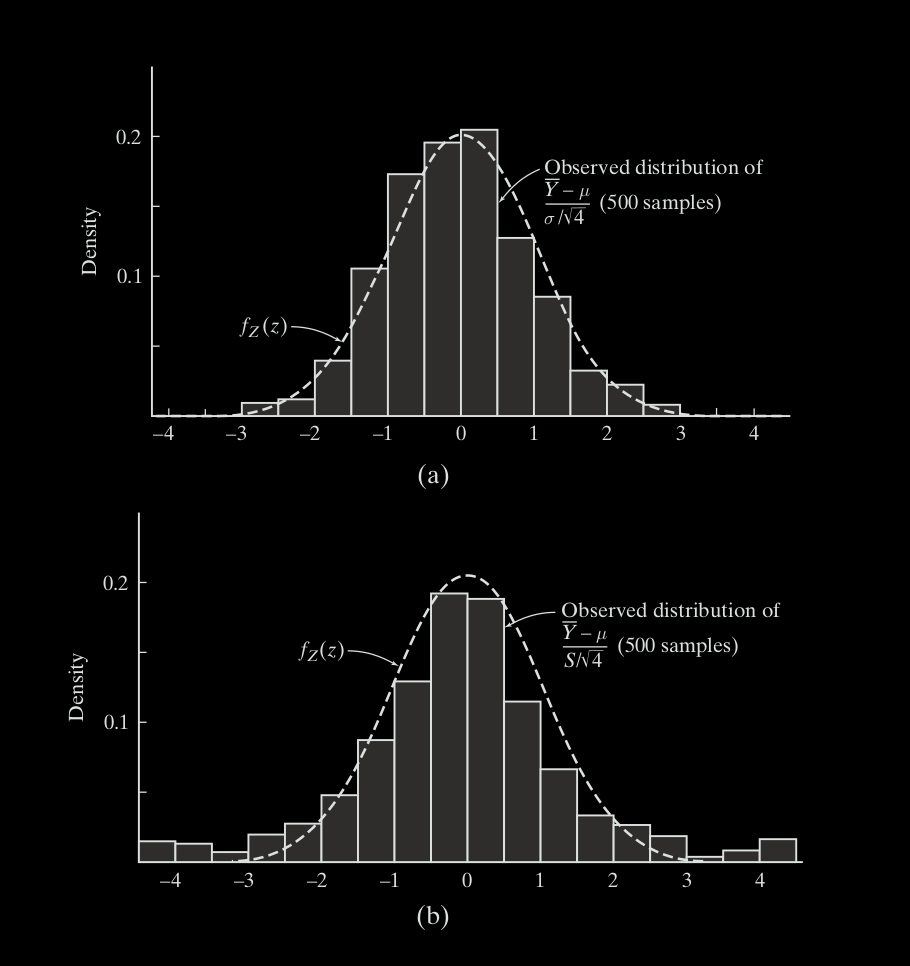
\includegraphics[scale=0.2]{Figure_7-2-1-neg.png}
	\end{center}
\end{frame}
%-------------- end slide -------------------------------%}}}
%-------------- start slide -------------------------------%{{{ 7.18
\begin{frame}
\centering
	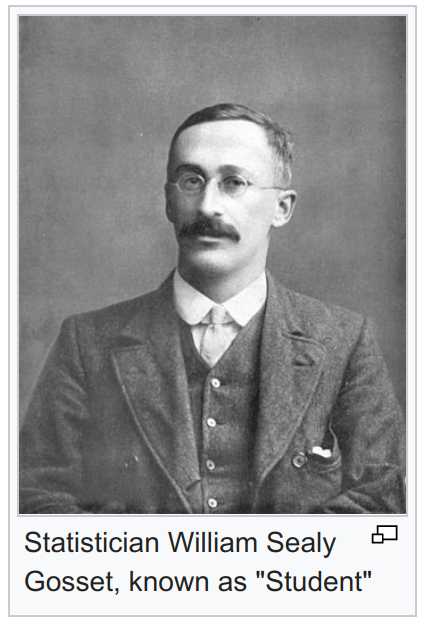
\includegraphics[scale=0.2]{Student.png}
	\hspace{3em}
	
\includegraphics[scale=0.15]{Free-Pint-of-Guinness.png}
	\vfill
\footnotesize
	\begin{enumerate}
		\item[Ref.] Student's t distribution comes from William Sealy Gosset's 1908 paper in Biometrika under the pseudonym "Student".
		\item[] Gosset worked at the Guinness Brewery in Dublin, Ireland, and was interested in the problems of small samples -- for example, the chemical properties of barley where sample sizes might be as few as 3.
		\item[V1] One version of the origin of the pseudonym is that Gosset's employer preferred staff to use pen names when publishing scientific papers instead of their real name, so he used the name "Student" to hide his identity.
	\item[V2] Another version is that Guinness did not want their competitors to know that they were using the t-test to determine the quality of raw material
	\end{enumerate}
\end{frame}
%-------------- end slide -------------------------------%}}}

\mySection{7.3 Deriving the Distribution of $\frac{\overline{Y}-\mu}{S/\sqrt{n}}$}
%-------------- start slide -------------------------------%{{{ 7.21
\begin{frame}
	% {\S\: 7.3 Deriving the Distribution of $\frac{\overline{Y}-\mu}{S/\sqrt{n}}$}
\begin{enumerate}
	\item[Def.] \textcolor{yellow!80!black}{\bf Sampling distributions}\\[1em]
		Distributions of \underline{\it functions of random sample} of given size.  \\
		\hspace{8.5em}  statistics / estimators
		\vfill
	\item[E.g.] A random sample of size $n$ from $N(\mu,\sigma^2)$ with $\sigma^2$ known.\\[1em]
		Sample mean $\overline{Y} = \frac{1}{n}\sum_{i=1}^n Y_i\sim N(\mu,\sigma^2/n)$
		\vfill
	\item[Aim:] Determine distributions for \\[2em]
		\begin{center}
			\begin{tabular}{c|c}
				Sample variance $S^2:=\frac{1}{n-1}\sum_{i=1}^n\left(Y_i-\overline{Y}\right)^2$ & {\it Chi square distr.}\\[1em]
				$\displaystyle T:=\frac{\overline{Y}-\mu}{S/\sqrt{n}}$ & {\it Student t distr.}\\[1em]
				$\displaystyle \frac{S_1^2}{\sigma_1^2}\bigg/\frac{S_2^2}{\sigma_2^2}$ & {\it F distr.}
			\end{tabular}
		\end{center}
\end{enumerate}
\end{frame}
%-------------- end slide -------------------------------%}}}
%-------------- start slide -------------------------------%{{{ 7.22
\begin{frame}
\begin{enumerate}
	\item[Thm \small 7.3.1.] Let $U=\sum_{i=1}^m Z_j^2$, where $Z_j$ are independent
		$N(0,1)$ normal r.v.s. Then
		\[
			\text{$U\sim$ Gamma(shape=$m/2$, rate=$1/2$).}
		\]
		namely,
		\[
			f_U(u) =  \frac{1}{2^{m/2}\Gamma(m/2)}u^{ \frac{m}{2}-1}e^{-u/2}, \qquad u\ge 0.
		\]
		\vfill
	\item[Def \small 7.3.1.] $U$ in Thm 7.3.1 is called \textcolor{yellow!80!black}{\bf chi square distribution} with $m$ dgs of freedom.
\end{enumerate}
\end{frame}
%-------------- end slide -------------------------------%}}}
%-------------- start slide -------------------------------%{{{ 7.23
\begin{frame}[fragile]
	\begin{enumerate}
		\item[Proof.] We first consider the case when $m=1$. In this case,
			\begin{align*}
				F_{Z^2}(u) & = \bbP\left(Z^2\le u\right)                     \\
                   & = \bbP\left( -\sqrt{u}\le Z \le \sqrt{u}\right) \\
                   & = 2 \bbP(0\le Z\le \sqrt{u})                    \\
                   & = \frac{2}{\sqrt{2\pi}} \int_0^{2\pi} e^{-z^2/2} \ud z
			\end{align*}
		\item[] Differentiating both sides of the above eq. in order to obtain the pdf:
			\begin{align*}
				f_{Z^2}(u) & = \frac{\ud}{\ud u} F_{Z^2}(u)                       \\
                   & = \frac{2}{\sqrt{2\pi}} \frac{1}{2\sqrt{u}} e^{-u/2} \\
                   & = \frac{1}{\sqrt{2} \Gamma(1/2)} u^{(1/2)-1} e^{-u/2},
			\end{align*}
		\item[] which is the pdf of a gamma distribution with $r=\lambda=1/2$.
		\item[] Then adding $m$ independent copies of gamma distributions gives anther gamma
			distribution with $r=m/2$ and $\lambda=1/2$ (See Theorem 4.6.4). \myEnd
	\end{enumerate}
\end{frame}
%-------------- end slide -------------------------------%}}}
%-------------- start slide -------------------------------%{{{ 7.24 Chi Square Table with R
\begin{frame}[fragile]{Chi Square Table}
\begin{center}
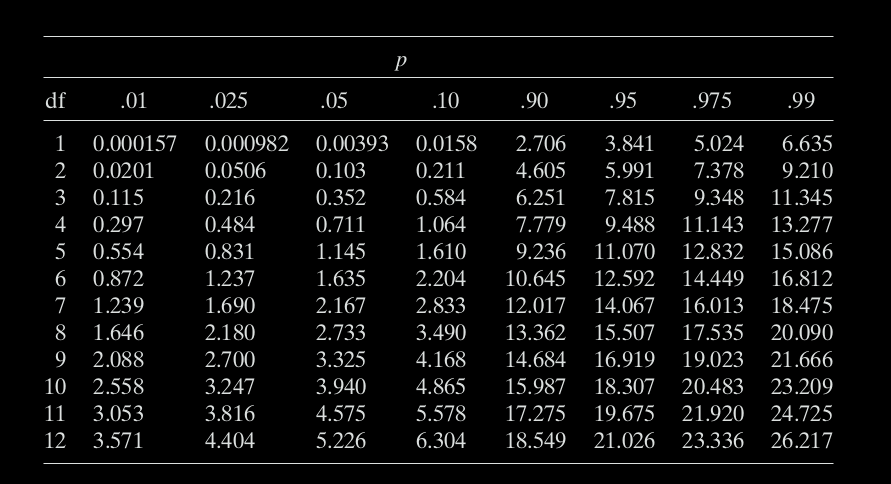
\includegraphics[scale=0.18]{Figure_7-5-2-neg.png}
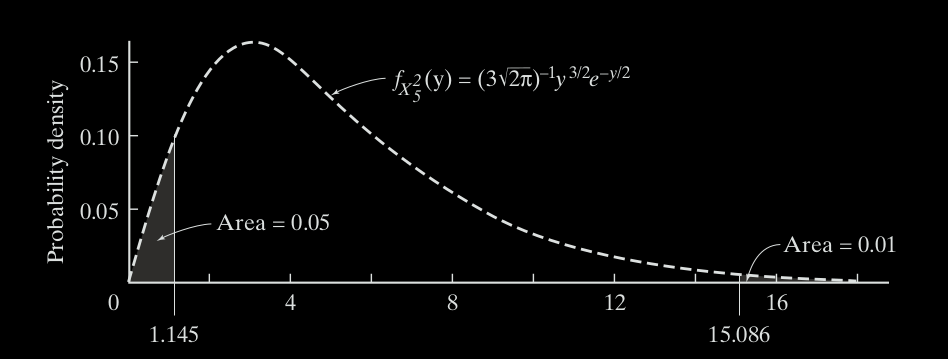
\includegraphics[scale=0.18]{Figure_7-5-1-neg.png}
\begin{align*}
	\bbP(\chi_5^2\le 1.145) = 0.05 & \quad \Longleftrightarrow  \quad \chi_{0.05,5}^2 =1.145 \\
	\bbP(\chi_5^2\le 15.086)=0.99  & \quad \Longleftrightarrow  \quad \chi_{0.99,5}^2 =15.086
\end{align*}
\begin{minipage}{0.3\textwidth}
\begin{lstlisting}
> pchisq(1.145, df = 5)
[1] 0.04995622
> pchisq(15.086, df = 5)
[1] 0.9899989
\end{lstlisting}
\end{minipage}
\qquad\qquad
\begin{minipage}{0.3\textwidth}
\begin{lstlisting}
> qchisq(0.05, df = 5)
[1] 1.145476
> qchisq(0.99, df = 5)
[1] 15.08627
\end{lstlisting}
\end{minipage}
\end{center}
\end{frame}
%-------------- end slide -------------------------------%}}}
%-------------- start slide -------------------------------%{{{ 7.24 Chi Square Table with Python
\begin{frame}[fragile]{Chi Square Table}
\begin{center}
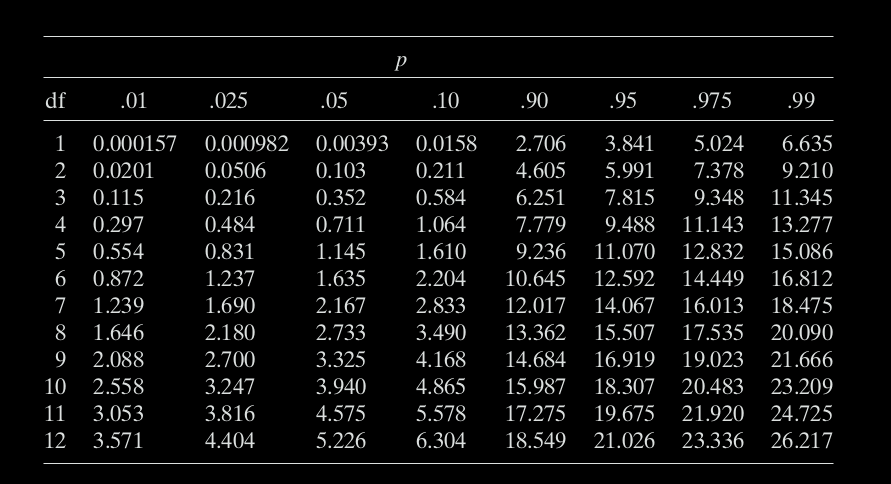
\includegraphics[scale=0.18]{Figure_7-5-2-neg.png}
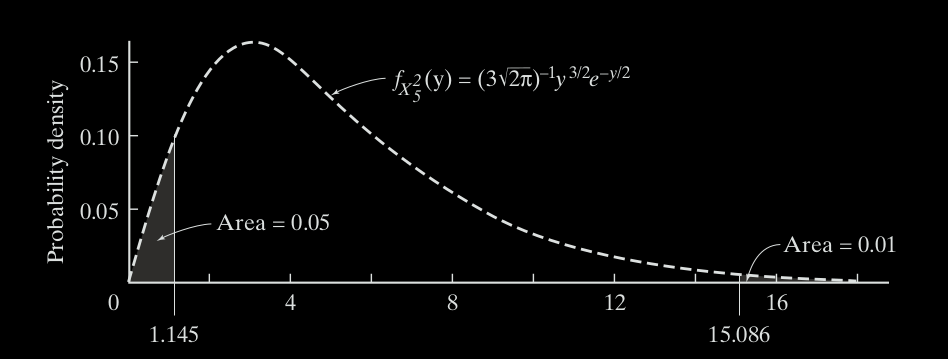
\includegraphics[scale=0.18]{Figure_7-5-1-neg.png}
\begin{align*}
	\bbP(\chi_5^2\le 1.145) = 0.05 & \quad \Longleftrightarrow  \quad \chi_{0.05,5}^2 =1.145 \\
	\bbP(\chi_5^2\le 15.086)=0.99  & \quad \Longleftrightarrow  \quad \chi_{0.99,5}^2 =15.086
\end{align*}
\begin{minipage}{0.4\textwidth}
\begin{lstlisting}[language=Python]
> scipy.stats.chi2.cdf(1.145, 5)
[1]: 0.04995622155207728
> scipy.stats.chi2.cdf(15.086, 5)
[1]: 0.9899988752378142
\end{lstlisting}
\end{minipage}
\begin{minipage}{0.4\textwidth}
\begin{lstlisting}[language=Python]
> scipy.stats.chi2.ppf(0.05, 5)
[1]: 1.1454762260617692
> scipy.stats.chi2.ppf(0.99, 5)
[1]: 15.08627246938899
\end{lstlisting}
\end{minipage}
\end{center}
\end{frame}
%-------------- end slide -------------------------------%}}}
%-------------- start slide -------------------------------%{{{ 7.25
\begin{frame}[fragile]
\begin{enumerate}
\item[Thm \small 7.3.2.] Let $Y_1,\cdots, Y_n$ be a random sample from $N(\mu,\sigma^2)$. Then
\item[] (a) $S^2$ and $\overline{Y}$ are independent.
\item[] (b) $\displaystyle \frac{(n-1)S^2}{\sigma^2} = \frac{1}{\sigma^2}\sum_{i=1}^n\left(Y_i-\overline{Y} \right)^2\quad \sim\quad$ Chi Square($n-1$).
\vfill
\item[Proof.] We will prove the case $n=2$.
	\[
	\overline{Y} =  \frac{Y_1+Y_2}{2},\qquad
Y_1-\overline{Y} =  \frac{Y_1-Y_2}{2}, \qquad
Y_2-\overline{Y} =  \frac{Y_2-Y_1}{2}
	\]
	\[
		S^2 = ...=  \frac{1}{2} \left( Y_1-Y_2 \right )^2
	\]
	\vfill
\item[(a)] It is equivalanet to show $Y_1+Y_2 \perp Y_1-Y_2$. Since they are normal, it suffices to show that
	\[
		\E[(Y_1+Y_2)(Y_1-Y_2)] =
		\E[Y_1+Y_2]
		\E[Y_1-Y_2]
	\]
	\vfill
\item[(b)] $\frac{(n-1)S^2}{\sigma^2} = \left(  \frac{Y_1-Y_2}{\sqrt{2}\sigma} \right)^2 $ and $\frac{Y_1-Y_2}{\sqrt{2}\sigma}\sim N(0,1)$ ...
	\myEnd
\end{enumerate}

\end{frame}
%-------------- end slide -------------------------------%}}}
%-------------- start slide -------------------------------%{{{ 7.26
\begin{frame}
\begin{enumerate}
\item[Def \small 7.3.2.] If $U\sim$ Chi Square$(n)$ and $V\sim$ Chi Square$(m)$, and $U\perp V$, then
\[
F:= \frac{V/m}{U/n}
\]
follows the \textcolor{yellow!80!black}{\bf (Snedecor's) F distribution} with $m$ and $n$ degrees of freedom.
\vfill
\item[Thm \small 7.3.3.] Let $F_{m,n}=\frac{V/m}{U/n}$ be an $F$ r.v. with $m$ and $n$ degrees of freedom. Then
\[
	f_{F_{m,n}}(w) =
	\frac{\Gamma\left(\frac{m+n}{2}\right)m^{m/2}n^{n/2}}{\Gamma(m/2)\Gamma(n/2)} \times
	\frac{w^{m/2-1}}{(n+mw)^{(m+n)/2}}, \quad w\ge 0
\]
\item[] Equivalently,
\[
	f_{F_{m,n}}(w)
	=
	B(m/2,n/2)^{-1} \left(\frac{m}{n} \right)^{\frac{m}{2}} w^{\frac{m}{2}-1}\left( 1+\frac{m}{n}w \right)^{-\frac{m+n}{2}}
\]
\item[] where $B(a,b)=\Gamma(a)\Gamma(b)/\Gamma(a+b)$.
\end{enumerate}
\end{frame}
%-------------- end slide -------------------------------%}}}
%-------------- start slide -------------------------------%{{{ 7.27
\begin{frame}
\begin{enumerate}
	\item[Recall] \phantom{a}\\
	% 	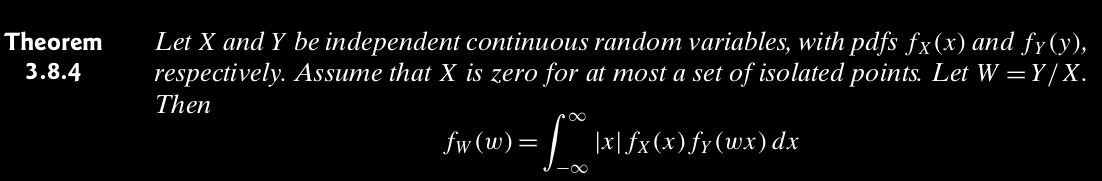
\includegraphics[scale=0.28]{Theorem-3-8-4-neg.png}
	\vfill
	\item[Thm \small 3.8.4] Let $X$ and $Y$ be independent continuous random variables, with
		pdf $f_X(x)$ and $f_Y(y)$, respectively.
	\item[] Assume that $X$ is zero for at most a set of isolated points.
	\item[] Then $W=Y/X$ follows a distribution with pdf:
		\begin{align*}
			f_W(w) = \int_{-\infty}^\infty |x| f_X(x) f_Y(wx) \ud x.
		\end{align*}
		\vfill
	\item[Thm \small 3.8.2] Suppose $X$ is a continuous random variable and $a\ne 0$.
	\item[] Then $Y=aX+b$ follows a distribution with pdf:
		\begin{align*}
			f_Y(y) = \frac{1}{|a|} f_X\left(\frac{y-b}{a}\right).
		\end{align*}
\end{enumerate}
\end{frame}
%-------------- end slide -------------------------------%}}}
%-------------- start slide -------------------------------%{{{ 7.28
\begin{frame}
	\begin{enumerate}
		\item[Proof.] Let us first find the pdf for $W:=V/U$. By Theorem 7.3.1,
			\begin{align*}
					f_V(v) & = \textcolor{yellow}{\frac{1}{2^{m/2}\Gamma(m/2)}v^{(m/2)-1}e^{-v/2}} ,\\
					f_U(u) & = \textcolor{lgtblue}{\frac{1}{2^{n/2}\Gamma(n/2)}u^{(n/2)-1}e^{-u/2}} .
			\end{align*}
		\vfill
		\item[] Then by Theorem 3.8.4, we see that the pdf of $W$ is
			\begin{align*}
				f_W(w) & = \int_{-\infty}^\infty \textcolor{magenta}{|u|} \textcolor{lgtblue}{f_U(u)} \: \textcolor{yellow}{f_V(uw)}\ud u \\
							 & = \int_0^\infty \textcolor{magenta}{u} \textcolor{lgtblue}{\frac{1}{2^{n/2}\Gamma(n/2)}u^{(n/2)-1}e^{-u/2}} \textcolor{yellow}{\frac{1}{2^{m/2}\Gamma(m/2)}(uw)^{(m/2)-1}e^{-uw/2}} \ud u\\
							 & = \frac{1}{2^{(n+m)/2}\Gamma(n/2)\Gamma(m/2)}w^{(m/2)-1}\int_0^\infty u^{\frac{n+m}{2}-1} e^{-\frac{1+w}{2} u}\ud u \\
			\end{align*}
	\end{enumerate}
\end{frame}
%-------------- end slide -------------------------------%}}}
%-------------- start slide -------------------------------%{{{ 7.29
\begin{frame}
	\begin{enumerate}
		\item[] Then by the change of variables, $y=\frac{1+w}{2}u$, we see that
			\begin{align*}
				f_W(w) & = \frac{1}{2^{(n+m)/2}\Gamma(n/2)\Gamma(m/2)}w^{(m/2)-1} \left(\frac{2}{1+w}\right)^{\frac{n+m}{2}} \int_0^\infty y^{\frac{n+m}{2}-1} e^{-y}\ud y \\
							 & = \frac{1}{2^{(n+m)/2}\Gamma(n/2)\Gamma(m/2)}w^{(m/2)-1}  \left(\frac{2}{1+w}\right)^{\frac{n+m}{2}} \Gamma\left(\frac{n+m}{2}\right)
			\end{align*}
			where the last equality is due to the definition of the Gamma function.
		\vfill
	\item[] Finally, by Theorem 3.8.2, we see that $F=\frac{V/m}{U/n} = \frac{n}{m} W$ follows a distribution with pdf
		\begin{align*}
			f_F(y) & = \frac{m}{n} f_W\left(\frac{m}{n} y\right)\\
             & = \textcolor{yellow}{\frac{m}{n}} \frac{1}{2^{(n+m)/2}\Gamma(n/2)\Gamma(m/2)}\left(\textcolor{yellow}{\frac{m}{n}y}\right)^{(m/2)-1} \left(\frac{2}{1+\textcolor{yellow}{\frac{m}{n}y}}\right)^{\frac{n+m}{2}} \Gamma\left(\frac{n+m}{2}\right) \\[1em]
             & = \cdots \qquad y \ge 0.
		\end{align*}
		\myEnd
	\end{enumerate}
\end{frame}
%-------------- end slide -------------------------------%}}}
%-------------- start slide -------------------------------%{{{ 7.30
\begin{frame}[fragile]
\begin{center}
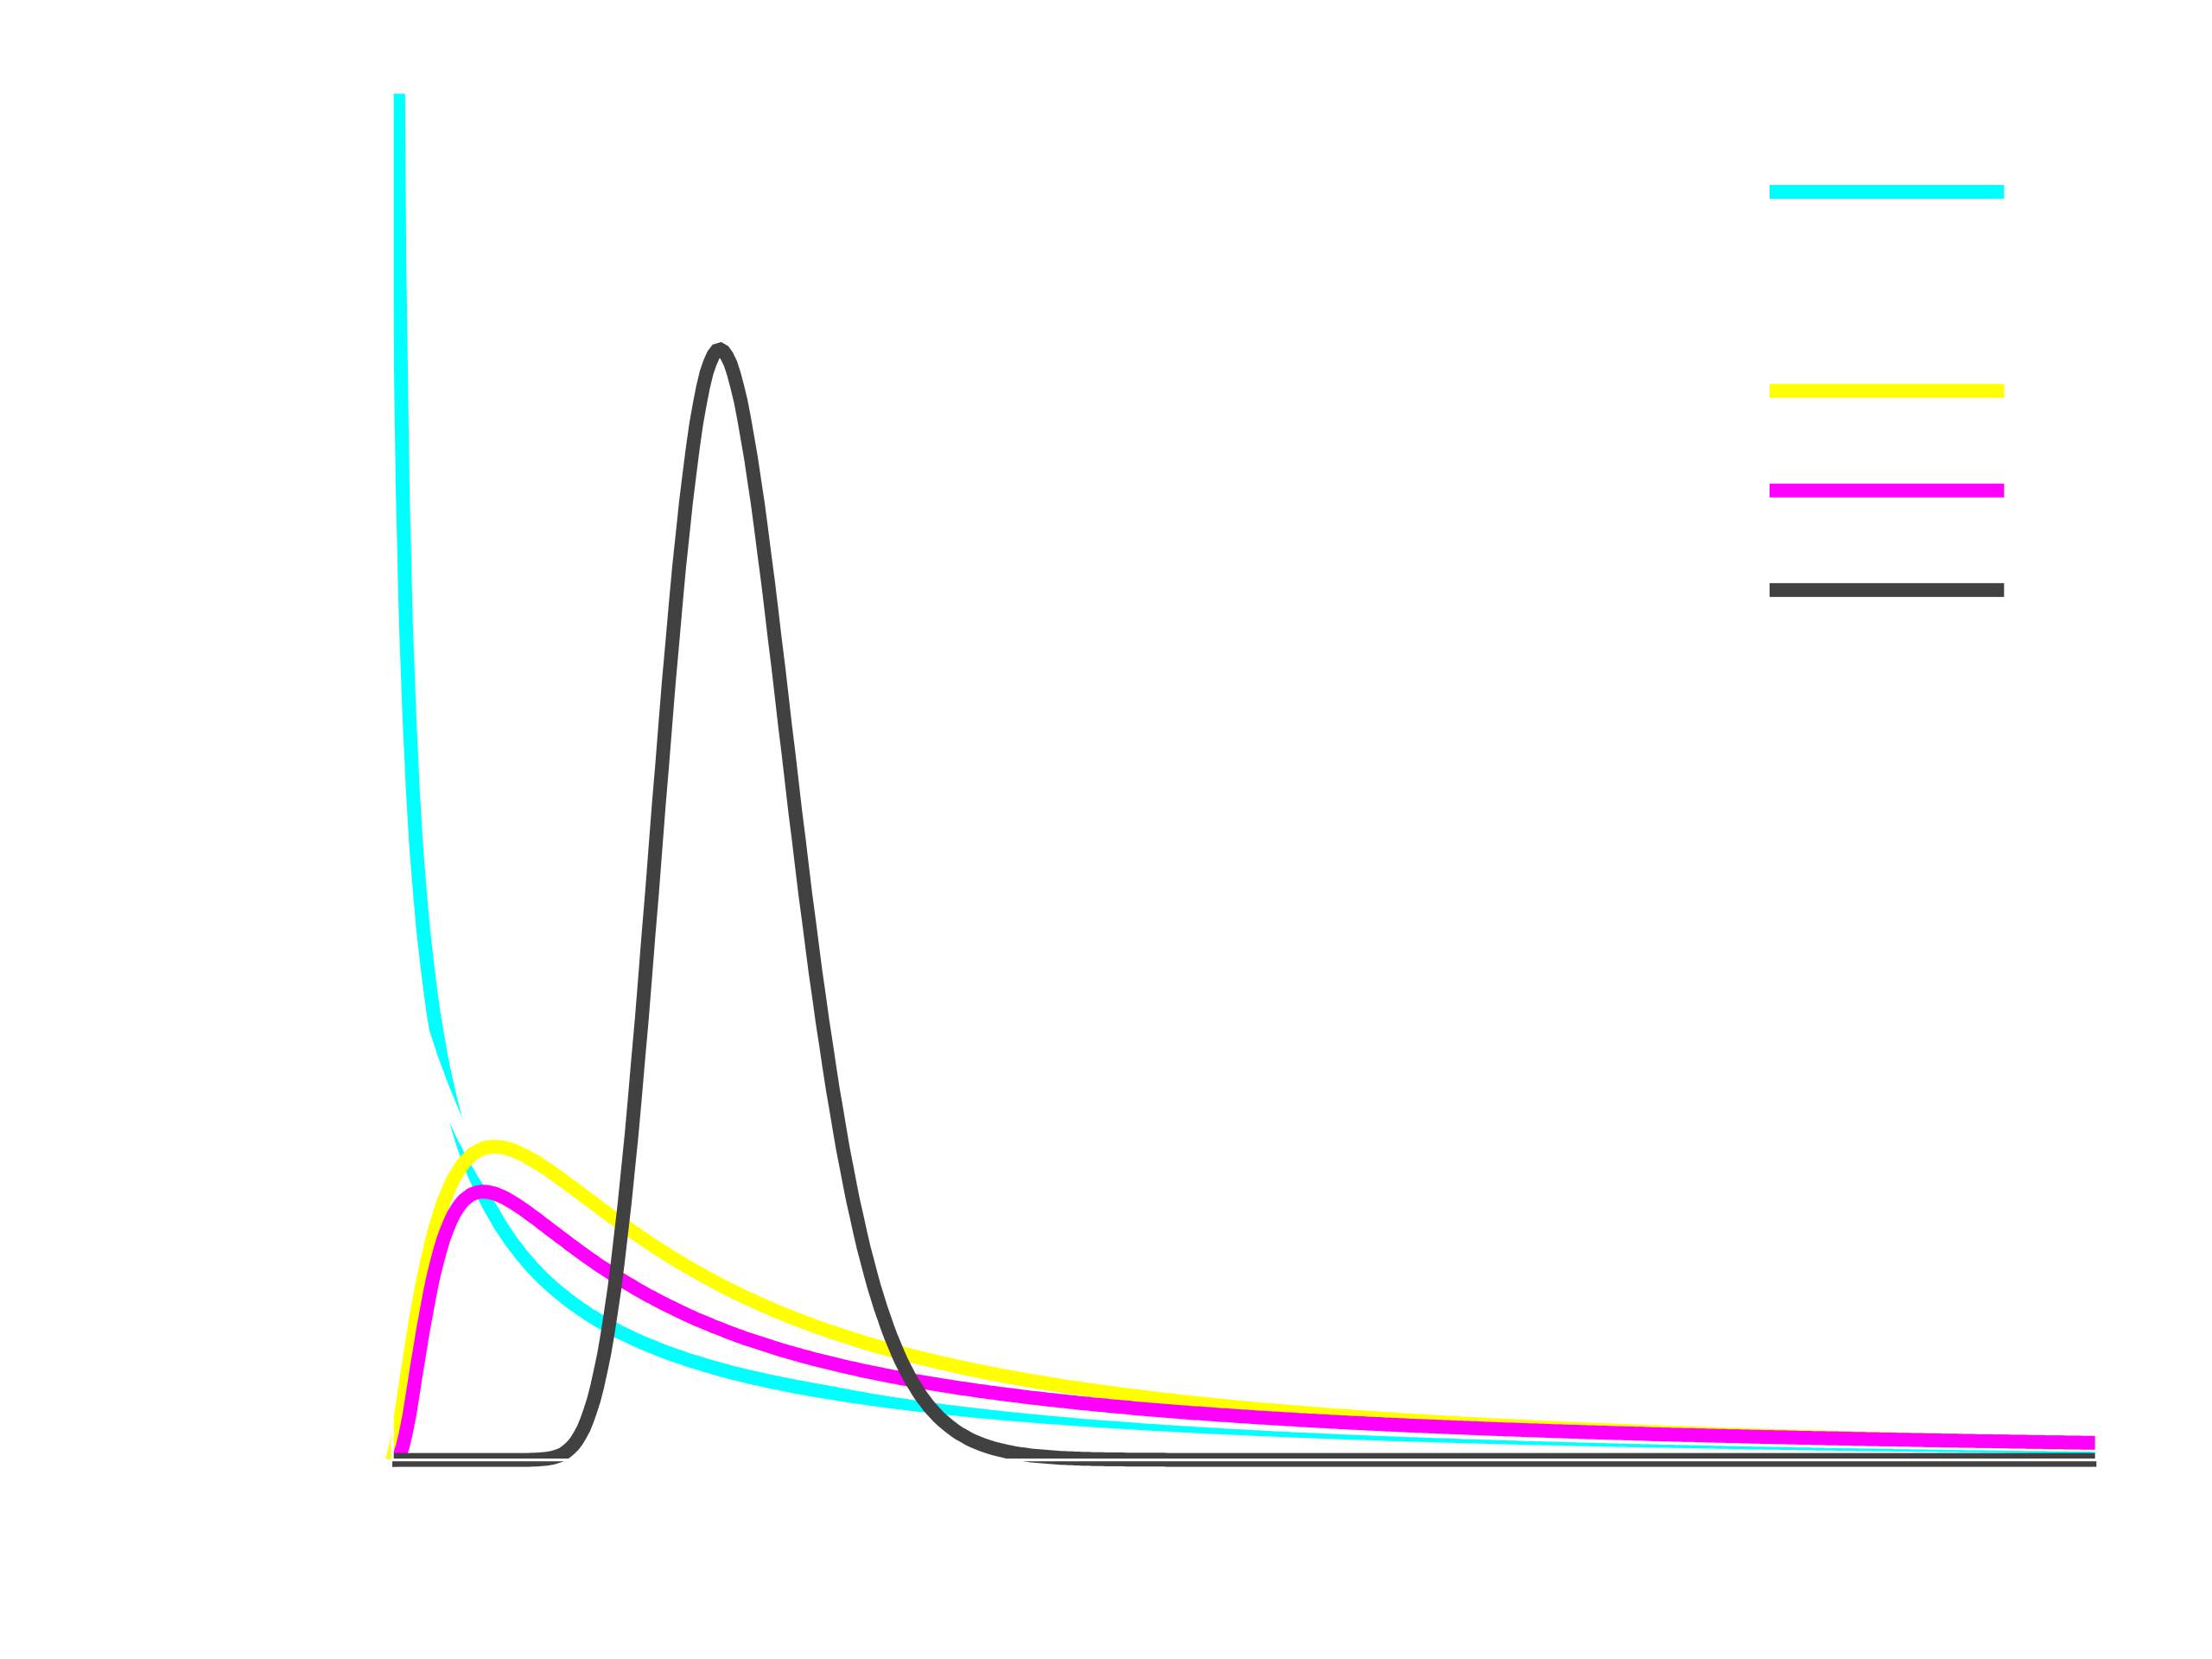
\includegraphics[scale=0.07]{F-distribution_pdf-neg.png}
\end{center}
\vfill
\begin{center}
\begin{minipage}{0.6\textwidth}
\begin{lstlisting}
# Draw F density
x=seq(0,5,0.01)
pdf= cbind(df(x, df1 = 1, df2 = 1),
df(x, df1 = 2, df2 = 1),
df(x, df1 = 5, df2 = 2),
df(x, df1 = 10, df2 = 1),
df(x, df1 = 100, df2 = 100))
matplot(x,pdf, type = "l")
title("F with various dgrs of freedom")
\end{lstlisting}
\end{minipage}
\end{center}
\end{frame}
%-------------- end slide -------------------------------%}}}
%-------------- start slide -------------------------------%{{{ 7.31
\begin{frame}[fragile]{F- Table}
\begin{center}
	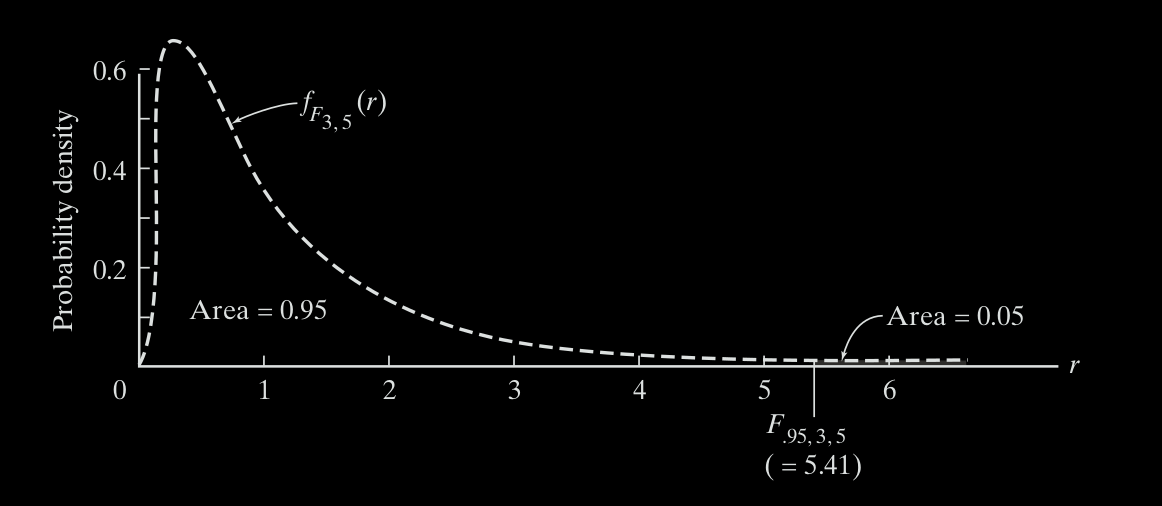
\includegraphics[scale=0.2]{Figure_7-3-1-neg.png}
	\[
		\bbP(F_{3,5}\le 5.41) = 0.95 \quad\Longleftrightarrow\quad
		F_{0.95,3,5} = 5.41
	\]
	\begin{minipage}{0.4\textwidth}
	\begin{lstlisting}
	> pf(5.41, df1 = 3, df2 = 5)
	[1] 0.9500093
	\end{lstlisting}
	\end{minipage}
	\qquad\qquad
	\begin{minipage}{0.4\textwidth}
	\begin{lstlisting}
	> qf(0.95, df1 = 3, df2 = 5)
	[1] 5.409451
	\end{lstlisting}
	\end{minipage}
	\vspace{-1em}

	\begin{minipage}{0.4\textwidth}
	\begin{lstlisting}
	> scipy.stats.f.cdf(5.41, 3, 5)
	[1] 0.9500092950699683
	\end{lstlisting}
	\end{minipage}
	\qquad\qquad
	\begin{minipage}{0.4\textwidth}
	\begin{lstlisting}
	> scipy.stats.f.ppf(0.95, 3, 5)
	[1] 5.40945131805649
	\end{lstlisting}
	\end{minipage}
\end{center}
\end{frame}
%-------------- end slide -------------------------------%}}}
%-------------- start slide -------------------------------%{{{ 7.32
\begin{frame}
\begin{enumerate}
\item[Def \small 7.3.3.] Suppose $Z\sim N(0,1)$, $U\sim$ Chi Square$(n)$, and $Z\perp U$.
Then
\[
T_n = \frac{Z}{\sqrt{U/n}}
\]
follows the \textcolor{yellow!80!black}{\bf Student's t-distribution} of $n$ degrees of freedom.
\vfill
\item[Remark] $T^2_n \sim F$-distribution with $1$ and $n$ degrees of freedom.
\vfill
\item[Thm \small 7.3.4.] The pdf of the Student t of degree $n$ is
\[
f_{T_n}(t) = \frac{\Gamma\left(\frac{n+1}{2} \right)}{\sqrt{n\pi}\Gamma\left(\frac{n}{2} \right)} \times \left(1+\frac{t^2}{n} \right)^{-\frac{n+2}{2}}, \quad t\in\R.
\]
% \vfill
% \item[Proof.] ... \myEnd
\end{enumerate}
\end{frame}
%-------------- end slide -------------------------------%}}}
% %-------------- start slide -------------------------------%{{{ 7.33
% \begin{frame}
% \centering
% 	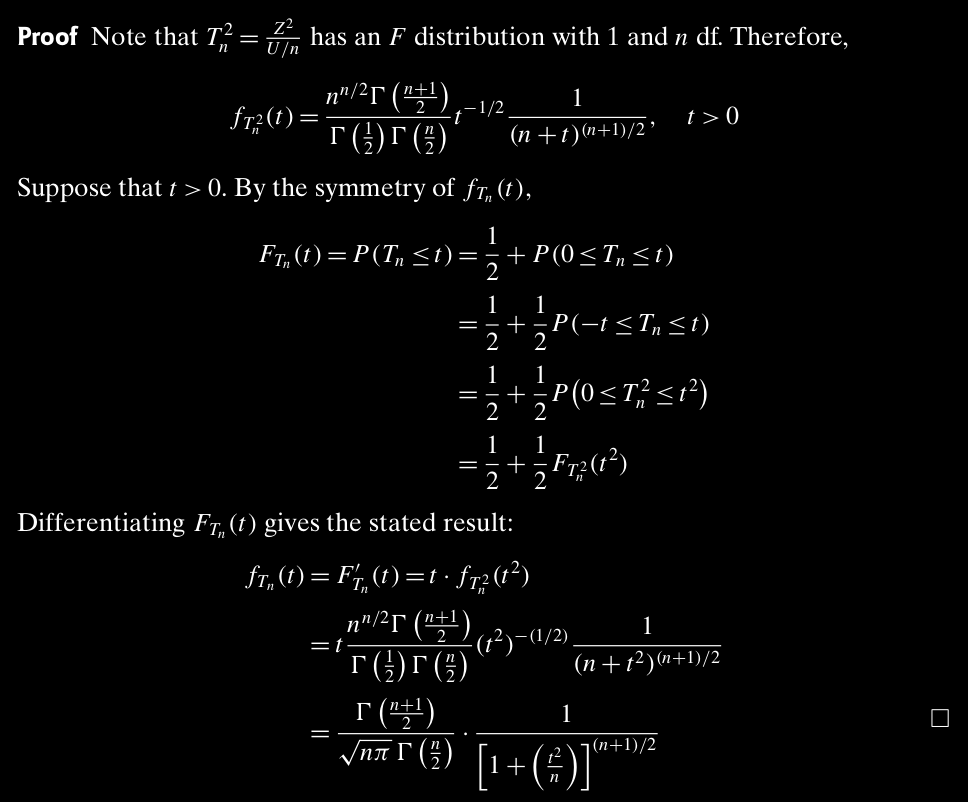
\includegraphics[scale=0.3]{Proof-Theorem-7-3-4-neg.png}
% \end{frame}
% %-------------- end slide -------------------------------%}}}
%-------------- start slide -------------------------------%{{{ 1
\begin{frame}[fragile]
\begin{itemize}
	\item[Proof.] Note that $T_n^2=\frac{Z^2}{U/n}$ follows an $F(1,n)$ distribution. Hence,
		\begin{align*}
			f_{T_n^2} (t) = \frac{n^{\frac{n}{2}}\Gamma(\frac{n+1}{2})}{\Gamma(\frac{1}{2})\Gamma(\frac{n}{2})} t^{-\frac{1}{2}} \frac{1}{(n+t)^{\frac{n+1}{2} }},\quad t> 0.
		\end{align*}
		\item[] Therefore,
		\begin{align*}
			F_{T_n}(t) & = \bbP(T_n\le t)  = \bbP(-\infty< T_n\le 0) + \bbP(0\le T_n\le t).
		\end{align*}
		\item[] The term $\bbP(-\infty< T_n\le 0)$ is a constant which will disappear upon differentiation.
		\item[] Notice that
		\begin{align*}
			\left\{T_n^2 \le t^2 \right\} & = \left\{-t \le T_n \le t\right\} = \left\{-t\le T_n \le 0\right\} \cup \left\{0\le T_n\le t\right\}\\
                                    & = \left\{-t \sqrt{U/n}\le Z \le 0\right\} \cup \left\{0\le Z\le t\sqrt{U/n}\right\}
		\end{align*}
\end{itemize}
\end{frame}
%-------------- end slide -------------------------------%}}}
%-------------- start slide -------------------------------%{{{ 1
\begin{frame}[fragile]
\begin{itemize}
	\item[]  By symmetry of the distribution of $Z$,
		\begin{align*}
			\bbP\left(-t \sqrt{U/n}\le Z \le 0\right)	= \bbP\left(0\le Z\le t\sqrt{U/n}\right)
		\end{align*}
		\item[] Therefore,
		\begin{align*}
			\bbP\left(T_n^2\le t^2\right) & = \bbP\left(-t \sqrt{U/n}\le Z \le 0\right)	+ \bbP\left(0\le Z\le t\sqrt{U/n}\right)\\
			& = 2 \bbP\left(0\le Z\le t\sqrt{U/n}\right)\\
			& = 2 \bbP(0\le T_n \le t).
		\end{align*}
		\item[] Hence,
		\begin{align*}
			F_{T_n}(t) &= const. + \frac{1}{2}\bbP\left(T_n^2\le t^2\right)
		\end{align*}
	\item[] Finally, differentiation gives the density:
	\begin{align*}
		f_{T_n}(t) & = \frac{d}{dt} F_{T_n}(t) = \frac{d}{dt} \frac{1}{2} F_{T_n^2}(t^2) = t\cdot  f_{T_n^2}(t^2) = \cdots .
	\end{align*}
	\myEnd
\end{itemize}
\end{frame}
%-------------- end slide -------------------------------%}}}
%-------------- start slide -------------------------------%{{{ 7.34
\begin{frame}[fragile]
\begin{center}
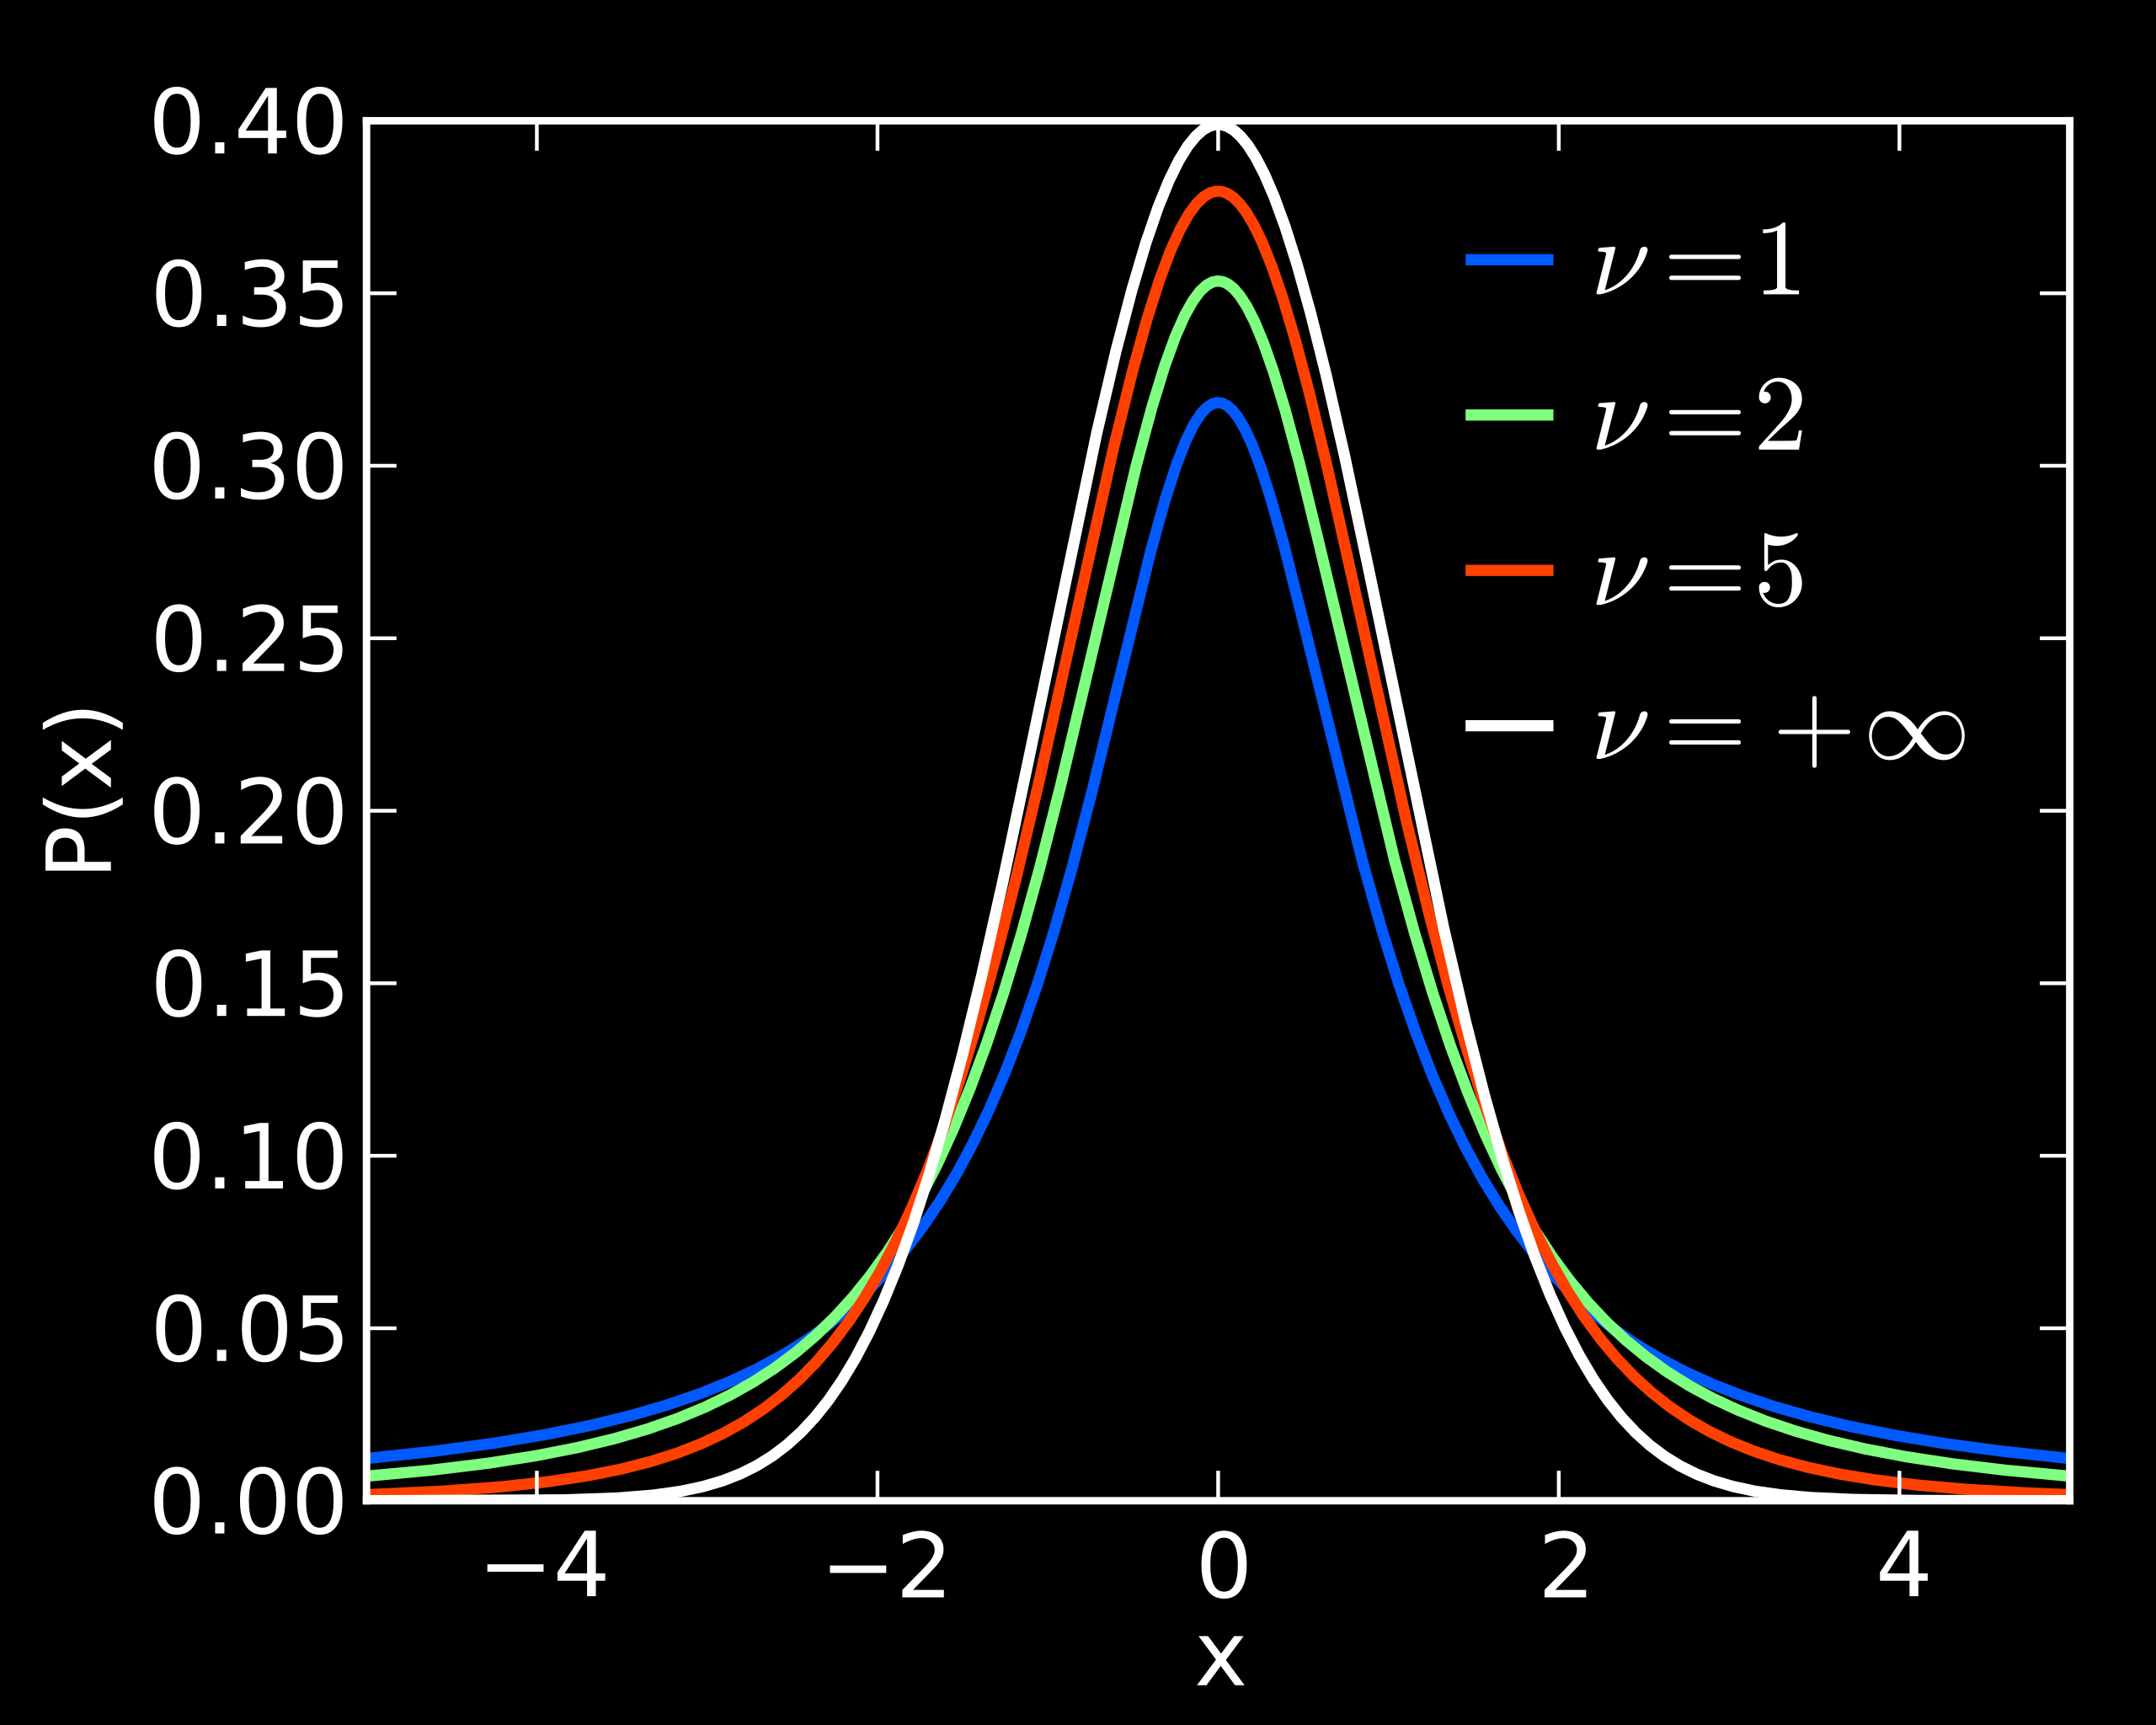
\includegraphics[scale=0.06]{Student_t_pdf-neg.png}\\
\vfill
\begin{minipage}{0.45\textwidth}
\begin{lstlisting}
# Draw Student t-density
x=seq(-5,5,0.01)
pdf= cbind(dt(x, df = 1),
	  			dt(x, df = 2),
	   			dt(x, df = 5),
	   			dt(x, df = 100))
matplot(x,pdf, type = "l")
title("Student's t-distributions")
\end{lstlisting}
\end{minipage}
\end{center}
\end{frame}
%-------------- end slide -------------------------------%}}}
%-------------- start slide -------------------------------%{{{ 7.35
\begin{frame}[fragile]{t Table}
\begin{center}
	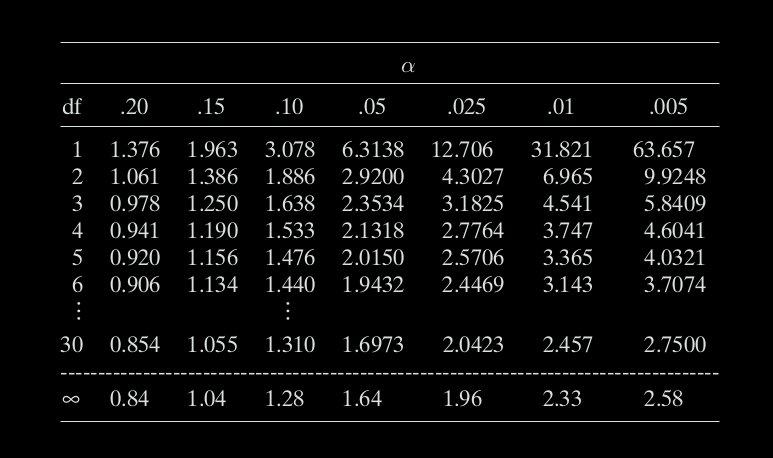
\includegraphics[scale=0.18]{Figure_7-4-1-neg.png}

	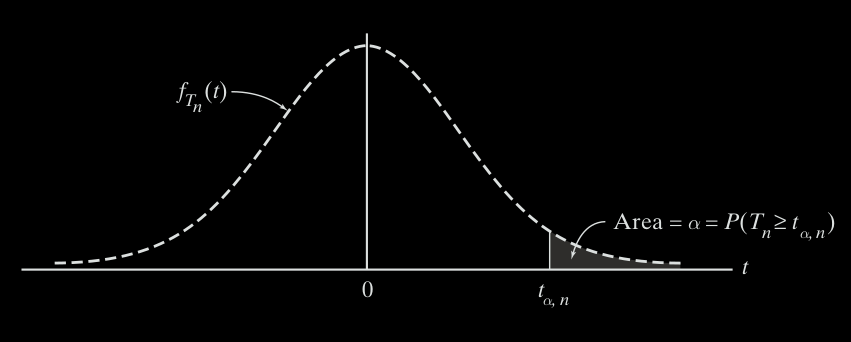
\includegraphics[scale=0.18]{Figure_7-4-2-neg.png}
	\[
		\bbP\left(T_3>4.541 \right) = 0.01 \quad \Longleftrightarrow \quad
		t_{0.01,3} = 4.541
	\]

	\begin{minipage}{0.4\textwidth}
	\begin{lstlisting}
	> 1-pt(4.541, df =3)
	[1] 0.009998238
	\end{lstlisting}
	\end{minipage}
	\qquad
	\begin{minipage}{0.4\textwidth}
	\begin{lstlisting}
	> alpha = 0.01
	> qt(1-alpha, df = 3)
	[1] 4.540703
	\end{lstlisting}
	\end{minipage}
  \vspace{-2em}

	\begin{minipage}{0.4\textwidth}
	\begin{lstlisting}[language=Python]
	> 1 - scipy.stats.t.cdf(4.541, 3)
	[1] 0.00999823806449407
	\end{lstlisting}
	\end{minipage}
	\qquad
	\begin{minipage}{0.4\textwidth}
	\begin{lstlisting}[language=Python]
	> scipy.stats.t.ppf(1-0.01, 3)
	[1] 4.540702858698419
	\end{lstlisting}
	\end{minipage}
\end{center}
\end{frame}
%-------------- end slide -------------------------------%}}}
%-------------- start slide -------------------------------%{{{ 7.36
\begin{frame}
\begin{enumerate}
	\item[Thm \small 7.3.5.] Let $Y_1,\cdots, Y_n$ be a random sample from $N(\mu,\sigma^2)$. Then
		\[
		T_{n-1} = \frac{\overline{Y}-\mu}{S/\sqrt{n}} \quad \sim \quad \text{Student's t of degree $n-1$.}
		\]
	\vfill
	\item[Proof.]
		\[
			\frac{\overline{Y}-\mu}{S/\sqrt{n}}  =  \frac{\displaystyle
				\frac{\overline{Y}-\mu}{\sigma/\sqrt{n}}
			}{
			\displaystyle
			\sqrt{ \frac{(n-1)S^2}{\sigma^2 (n-1)}}
		}
		\]
		\pause\\[1em]
		\[
			\frac{\overline{Y}-\mu}{\sigma/\sqrt{n}}\sim N(0,1)\qquad \perp \qquad
		\frac{(n-1)S^2}{\sigma^2}
		\sim \text{Chi Square$(n-1)$}
		\]
	\\[2em]
	\item[] By Def. 7.3.3 ... \myEnd
\end{enumerate}
\end{frame}
%-------------- end slide -------------------------------%}}}
%-------------- start slide -------------------------------%{{{ 7.37
\begin{frame}
\begin{enumerate}
\item[] As $n\rightarrow \infty$, Students' t distribution will converge to $N(0,1)$: \\
	\begin{center}
		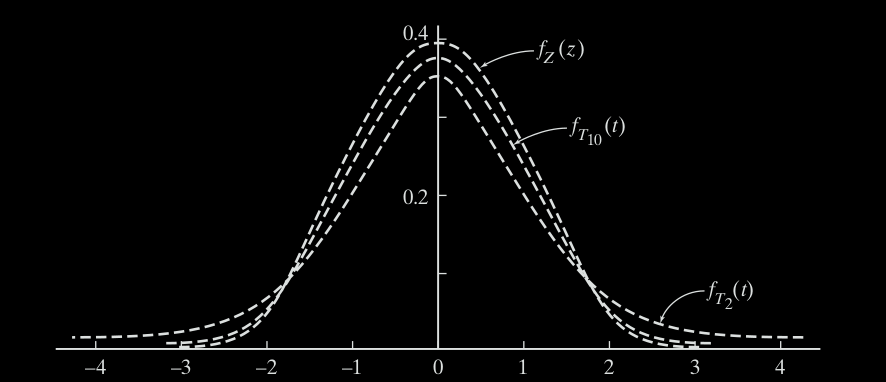
\includegraphics[scale=0.2]{Figure_7-3-2-neg.png}
	\end{center}
\vfill
\item[Thm \small 7.3.6.] $\displaystyle f_{T_n}(x)\rightarrow f_Z(x)= \frac{1}{\sqrt{2\pi}}e^{- \frac{x^2}{2}}\quad $ as $n\rightarrow\infty$, where $Z\sim N(0,1)$.
	\vfill
\item[Proof] By Stirling's formula:
	\[\Gamma(z) =\sqrt{ \frac{2\pi}{z}}\left( \frac{z}{e}\right)^z \left( 1+O(1/z) \right)
		\qquad\text{	as $z\rightarrow\infty$}
	\]
\item[]
	\[
		\Longrightarrow \quad \lim_{n\rightarrow\infty}  \frac{\Gamma\left(  \frac{n+1}{2} \right)}{\sqrt{n \pi}\: \Gamma\left(  \frac{n}{2} \right) } =  \frac{1}{\sqrt{2\pi}}
	\]
	......
	\myEnd
\end{enumerate}
\end{frame}
%-------------- end slide -------------------------------%}}}

\mySection{7.4  Drawing Inferences About $\mu$}
%-------------- start slide -------------------------------%{{{ 7.39
\begin{frame}
	% {\S\: 7.4  Drawing Inferences About $\mu$}
\begin{enumerate}
	\item[] Let $Y_1,\cdots,Y_n$ be a random sample from $N(\mu,\sigma^2)$.\\[1em]
	\item[Question] Find a test statistic $\Lambda$ in order to test\qquad $H_0 : \mu = \mu_0$ v.s. $H_1 : \mu \ne \mu_0$.
\vfill
\item[Case I.] $\sigma^2$ is known: \hspace{4em}
	$\displaystyle	\Lambda =  \frac{\overline{Y}-\mu_0}{\sigma/\sqrt{n}}$
\vfill
\item[Case II.] $\sigma^2$ is unknown: \hspace{3em} $\displaystyle \Lambda = \alert{?}$
	\pause \hspace{3em}
	$\displaystyle	\Lambda \stackrel{\alert{?}}{=}  \frac{\overline{Y}-\mu_0}{s/\sqrt{n}}\quad \sim\quad \alert{?}$
\end{enumerate}
\end{frame}
%-------------- end slide -------------------------------%}}}
%-------------- start slide -------------------------------%{{{ 7.40
\begin{frame}{Summary}
\begin{center}
A random sample of size $n$ from \\
a normal distribution $N(\mu,\sigma^2)$\\[2em]
\def\arraystretch{2}
\small
\begin{tabular}{c|c|c}
& $\sigma^2$ known & $\sigma^2$ unknown \\
\hline\hline
Statistic &
$Z = \frac{\overline{Y}-\mu}{\sigma/\sqrt{n}}$ &
$T_{n-1} = \frac{\overline{Y}-\mu}{S/\sqrt{n}}$\\
\hline
Score &
$z = \frac{\overline{y}-\mu}{\sigma/\sqrt{n}}$ &
$t = \frac{\overline{y}-\mu}{s/\sqrt{n}}$\\
\hline
Table & $z_{\alpha}$ & $t_{\alpha,n-1}$ \\
\hline
$100(1-\alpha)\%$ C.I. &
$\left( \bar{y}-z_{\alpha/2}\frac{\sigma}{\sqrt{n}}, \bar{y}+z_{\alpha/2}\frac{\sigma}{\sqrt{n}}\right)$ &
$\left( \bar{y}-t_{\alpha/2,n-1}\frac{s}{\sqrt{n}}, \bar{y}+t_{\alpha/2,n-1}\frac{s}{\sqrt{n}}\right)$ \\
\hline
Test $H_0:\mu=\mu_0$ &
&
\\
$H_1:\mu>\mu_0$ &   Reject $H_0$ if $z\ge z_{\alpha}$
&   Reject $H_0$ if $t\ge t_{\alpha,n-1}$
\\
$H_1:\mu<\mu_0$ &  Reject $H_0$ if $z\le z_{\alpha}$
&  Reject $H_0$ if $t\le t_{\alpha,n-1}$
\\
$H_1:\mu\ne\mu_0$ &  Reject $H_0$ if $|z|\ge z_{\alpha/2}$
&    Reject $H_0$ if $|t|\ge t_{\alpha/2,n-1}$
\\
\hline
\end{tabular}
\end{center}
\end{frame}
%-------------- end slide -------------------------------%}}}
%-------------- start slide -------------------------------%{{{ 7.41
\begin{frame}{Computing $s$ from data}
\begin{enumerate}
	\item[Step 1] $\displaystyle a=\sum_{i=1}^n y_i$
	\item[Step 2.] $\displaystyle b=\sum_{i=1}^n y_i^2$
	\item[Step 3.] $\displaystyle s =\sqrt{\frac{n b-a^2}{n(n-1)} } $
\vfill
\item[Proof.]\[
s^2 = \frac{1}{n-1}\sum_{i=1}^n (y_i-\bar{y})^2  =
\frac{n\left(\sum_{i=1}^n y_i^2\right) -\left(\sum_{i=1}^n y_i \right)^2}{n(n-1)}
\]
\myEnd
\end{enumerate}
\end{frame}
%-------------- end slide -------------------------------%}}}
%-------------- start slide -------------------------------%{{{ 7.42 Case 7.4.1
\begin{frame}
\begin{enumerate}
	\item[Case \small 7.4.1] How far apart are the bat and the insect when the bat first senses that insect is there? \\
	\item[] Or, what is the effective range of a bat's echolocation system?
		\begin{center}
		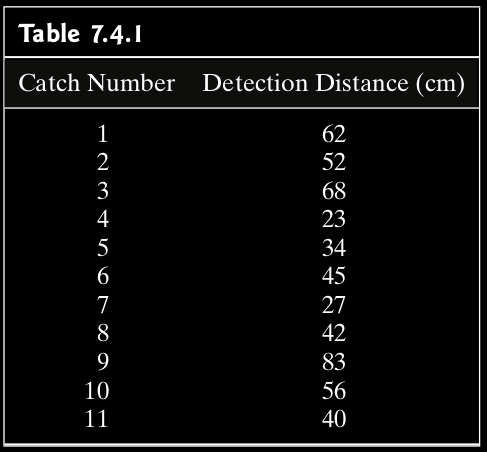
\includegraphics[scale=0.25]{Table_7-4-1-neg.png}
		\end{center}
	\item[] Answer the question by contruct a 95\% C.I.
\vfill
\item[Sol.] ... \myEnd
\end{enumerate}
\end{frame}
%-------------- end slide -------------------------------%}}}
%-------------- start slide -------------------------------%{{{ 1
\begin{frame}[fragile]
	\begin{lstlisting}[language=Python]
# Case7_4_1.py
import numpy as np
import scipy.stats as st


# returns confidence interval of mean
def confIntMean(a, conf=0.95):
    mean, sem, m = np.mean(a), st.sem(a), st.t.ppf((1+conf)/2., len(a)-1)
    return mean - m*sem, mean + m*sem


def main():
    alpha = 5
    data = np.array([62, 52, 68, 23, 34, 45, 27, 42, 83, 56, 40])
    lower, upper = confIntMean(data, 1-alpha/100)
    print("""\

    The {alpha}% confidence interval is ({lower:.2f},{upper:.2f})

        """.format(**locals()))


if __name__ == "__main__":
    main()
	\end{lstlisting}
	\begin{lstlisting}[language=Python]
In [83]: run Case7_4_1.py

    The 95% confidence interval is (36.21,60.51)


	\end{lstlisting}
\end{frame}
%-------------- end slide -------------------------------%}}}

%-------------- start slide -------------------------------%{{{ 7.43
\begin{frame}
	\begin{enumerate}
		\item[Eg. \small 7.4.2] Bank approval rates for inner-city residents v.s. rural ones.\\
		\item[] Approval rate for rural residents is 62\%.\\
		\item[] Do bank treat two groups equally? $\alpha=0.05$
			\begin{center}
				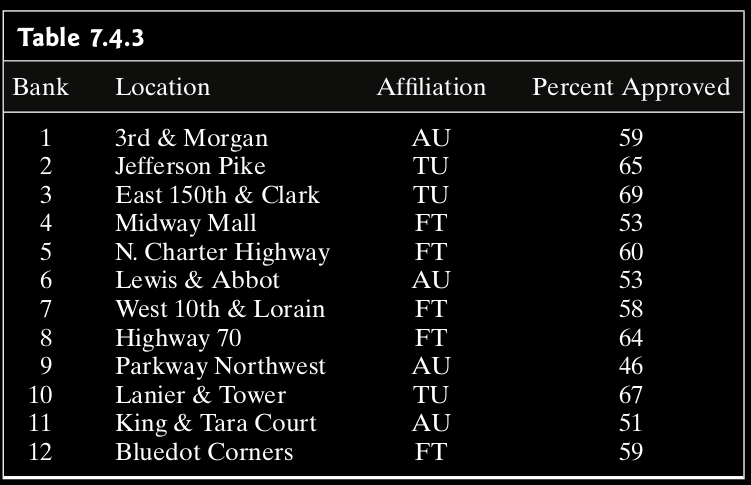
\includegraphics[scale=0.25]{Table_7-4-3-neg.png}
			\end{center}
		\vfill
		\item[Sol.]
			\[
			H_0: \mu = 62\qquad v.s. \qquad H_1: \mu \ne 62.
			\]
	\end{enumerate}
\end{frame}
%-------------- end slide -------------------------------%}}}
%-------------- start slide -------------------------------%{{{ 7.44
\begin{frame}
\centering
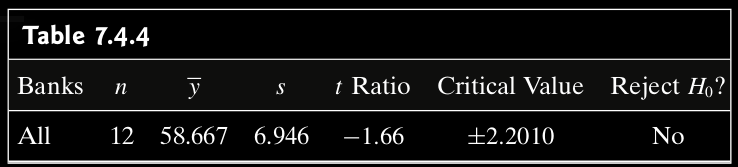
\includegraphics[scale=0.25]{Table_7-4-4-neg.png}
\vfill
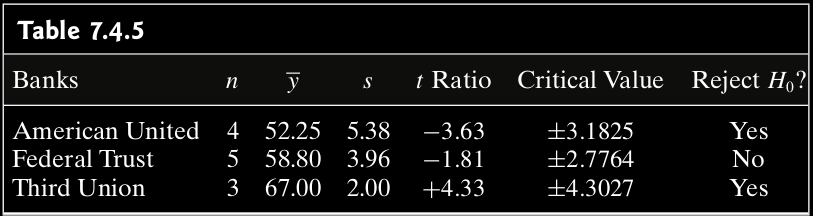
\includegraphics[scale=0.25]{Table_7-4-5-neg.png}
\end{frame}
%-------------- end slide -------------------------------%}}}
%-------------- start slide -------------------------------%{{{ 1 Codes for Eg 7.4.2
\begin{frame}[fragile]
\begin{lstlisting}[language=Python]
# Eg7_4_2.py
import numpy as np
import scipy.stats as st

data = np.array([59, 65, 69, 53, 60, 53, 58, 64, 46, 67,  51, 59])
alpha = 5
mean, sem = np.mean(data), st.sem(data)
n = len(data)
s = sem * np.sqrt(n)
cv = st.t.ppf(1-alpha/200., len(data)-1)
tRatio = (mean-62)/sem


print("""\

      n={n}, sample mean={mean:.3f}, s={s:.3f}, t Ratio={tRatio:.2f}, Critical values={cv:.4f}
      """.format(**locals()))
\end{lstlisting}
\begin{lstlisting}[language=Python]
In [113]: run Eg7_4_2.py

      n=12, sample mean=58.667, s=6.946, t Ratio=-1.66, Critical values=2.2010

\end{lstlisting}
\end{frame}
%-------------- end slide -------------------------------%}}}


\mySection{7.5  Drawing Inferences About $\sigma^2$}
%-------------- start slide -------------------------------%{{{ 7.47
\begin{frame}
	% {\S\: 7.5  Drawing Inferences About $\sigma^2$}
\begin{itemize}
	\item[]  For a random sample of size $n$ from $N(\mu,\sigma^2)$:
	\begin{align*}
	&S^2 =\frac{1}{n-1}\sum_{i=1}^n \left(Y_i-\overline{Y}\right)^2
	\pause \\ &\hspace{5em} \Downarrow\\
	&\frac{(n-1)S^2}{\sigma^2} = \frac{1}{\sigma^2}\sum_{i=1}^n \left(Y_i-\overline{Y}\right)^2
	\sim \text{Chi Square}(n-1)
	\end{align*}
	\item[] \pause
	\[
	\bbP\left(\chi_{\alpha/2,n-1}^2 \le \frac{(n-1)S^2}{\sigma^2}\le \chi_{1-\alpha/2,n-1}^2 \right)=1-\alpha.
	\]
\end{itemize}
\vfill
\pause
\begin{minipage}{0.45\textwidth}
	\centering
	$100(1-\alpha)\%$ C.I. for $\sigma^2$:
	\[
		\left(\frac{(n-1)s^2}{\chi^2_{1-\alpha/2,n-1}},  \frac{(n-1)s^2}{\chi^2_{\alpha/2,n-1}}\right)
	\]
\end{minipage}
\quad
\begin{minipage}{0.45\textwidth}
	\centering
	$100(1-\alpha)\%$ C.I. for $\sigma$:
	\[
		\left(\sqrt{\frac{(n-1)s^2}{\chi^2_{1-\alpha/2,n-1} }},  \sqrt{\frac{(n-1)s^2}{\chi^2_{\alpha/2,n-1} }}\right)
	\]
\end{minipage}
\end{frame}
%-------------- end slide -------------------------------%}}}
%-------------- start slide -------------------------------%{{{ 7.48
\begin{frame}
\centering
Testing $H_0:\sigma^2 = \sigma_0^2$ \\[1em] v.s.\\[1em]
(at the $\alpha$ level of significance)
\\[1em]
$\chi^2 = \frac{(n-1)s^2}{\sigma_0^2}$
\vfill

\begin{minipage}{0.32\textwidth}
\centering
$H_1:\sigma^2<\sigma_0^2$:\\[1em]
Reject $H_0$ if \\[1em]
$\chi^2 \le \chi_{\alpha,n-1}^2$
\end{minipage}
\begin{minipage}{0.32\textwidth}
\centering
$H_1:\sigma^2\ne \sigma_0^2$:\\[1em]
Reject $H_0$ if \\[1em]
$\chi^2 \le \chi_{\alpha/2,n-1}^2$ or \\[1em]
$\chi^2 \ge \chi_{1-\alpha/2,n-1}^2$
\end{minipage}
\begin{minipage}{0.32\textwidth}
\centering
$H_1:\sigma^2>\sigma_0^2$:\\[1em]
Reject $H_0$ if \\[1em]
$\chi^2 \ge \chi_{1-\alpha,n-1}^2$
\end{minipage}
\end{frame}
%-------------- end slide -------------------------------%}}}
%-------------- start slide -------------------------------%{{{ 7.49
\begin{frame}

\begin{enumerate}
\item[E.g. 1.] The width of a confidence interval for $\sigma^2$ is a function of $n$ and $S^2$:
\[
W=\frac{(n-1)S^2}{\chi^2_{\alpha/2,n-1}}-\frac{(n-1)S^2}{\chi^2_{1-\alpha/2,n-1}}
\]
Find the smallest $n$ such that the average width of a $95\%$ C.I. for $\sigma^2$ is no greater than $0.8 \sigma^2$.
\vfill
\item[Sol.] Notice that $\E[S^2]=\sigma^2$. Hence, we need to find $n$ s.t.
	\[
		(n-1)\left(\frac{1}{\chi_{0.025,n-1}^2} - \frac{1}{\chi_{0.975,n-1}^2}\right)\le 0.8.
	\]
\item[] Trial and error (numerics on R) gives $n=57$.
\end{enumerate}
\end{frame}
%-------------- end slide -------------------------------%}}}
%-------------- start slide -------------------------------%{{{ 7.50
\begin{frame}[fragile]
\begin{center}
\begin{minipage}{0.6\textwidth}
\begin{lstlisting}
> # Example 7.5.1
> n=seq(45,60,1)
> l=qchisq(0.025,n-1)
> u=qchisq(0.975,n-1)
> e=(n-1)* (1/l-1/u)
> m=cbind(n,l,u,e)
> colnames(m) = c("n",
+                 "chi(0.025,n-1)",
+                 "chi(0.975,n-1)",
+                 "error")
> m
       n chi(0.025,n-1) chi(0.975,n-1)     error
 [1,] 45       27.57457       64.20146 0.9103307
 [2,] 46       28.36615       65.41016 0.8984312
 [3,] 47       29.16005       66.61653 0.8869812
 [4,] 48       29.95620       67.82065 0.8759533
 [5,] 49       30.75451       69.02259 0.8653224
 [6,] 50       31.55492       70.22241 0.8550654
 [7,] 51       32.35736       71.42020 0.8451612
 [8,] 52       33.16179       72.61599 0.8355901
 [9,] 53       33.96813       73.80986 0.8263340
[10,] 54       34.77633       75.00186 0.8173761
[11,] 55       35.58634       76.19205 0.8087008
[12,] 56       36.39811       77.38047 0.8002937

[13,] 57       37.21159       78.56716 0.7921414
[14,] 58       38.02674       79.75219 0.7842313
[15,] 59       38.84351       80.93559 0.7765517
[16,] 60       39.66186       82.11741 0.7690918
\end{lstlisting}
\end{minipage}
	\end{center}
\end{frame}
%-------------- end slide -------------------------------%}}}
%-------------- start slide -------------------------------%{{{ 7.51
\begin{frame}
\centering
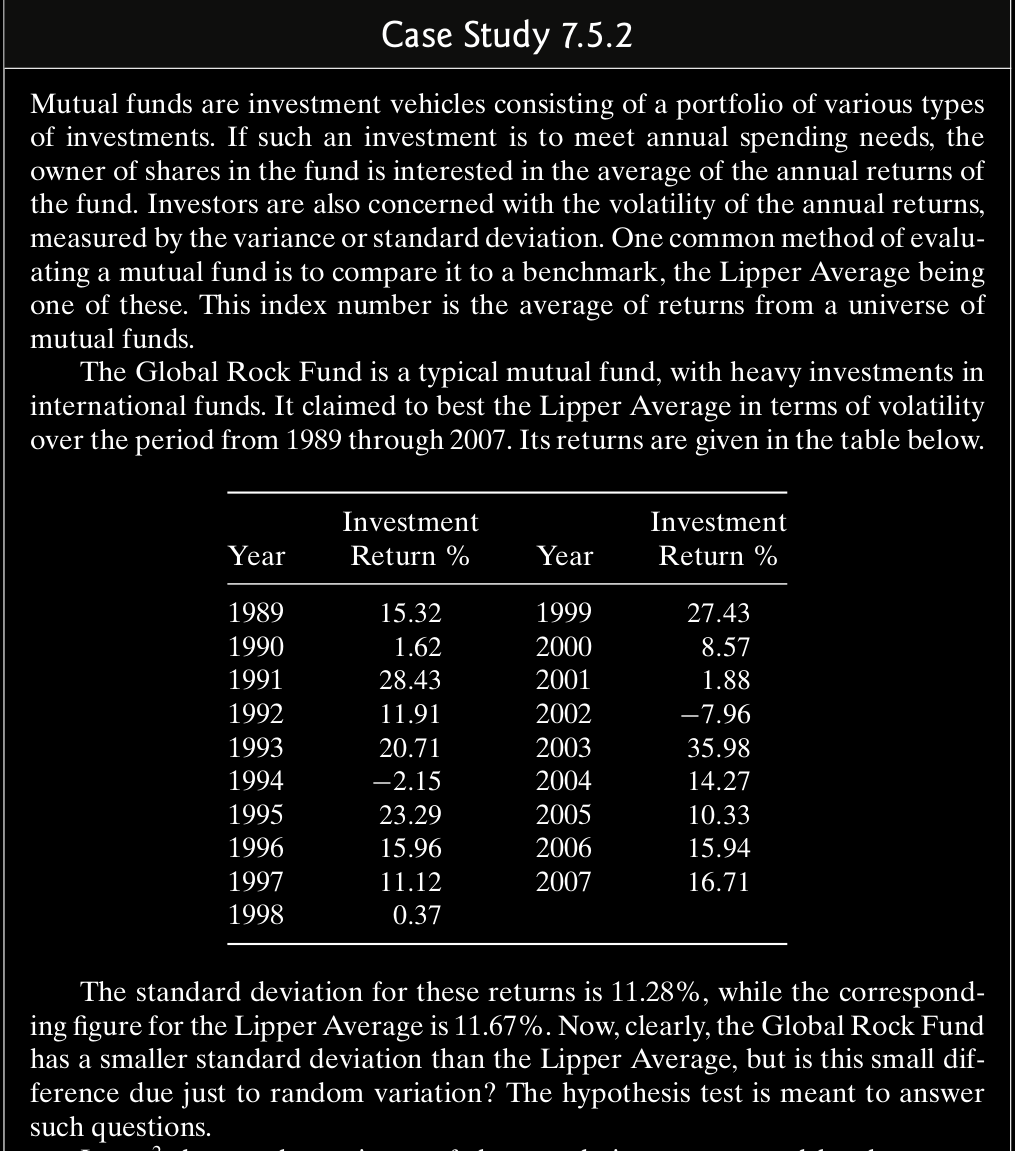
\includegraphics[scale=0.23]{Case_7-5-2-neg.png}
\end{frame}
%-------------- end slide -------------------------------%}}}
%-------------- start slide -------------------------------%{{{ 7.52
\begin{frame}
\centering
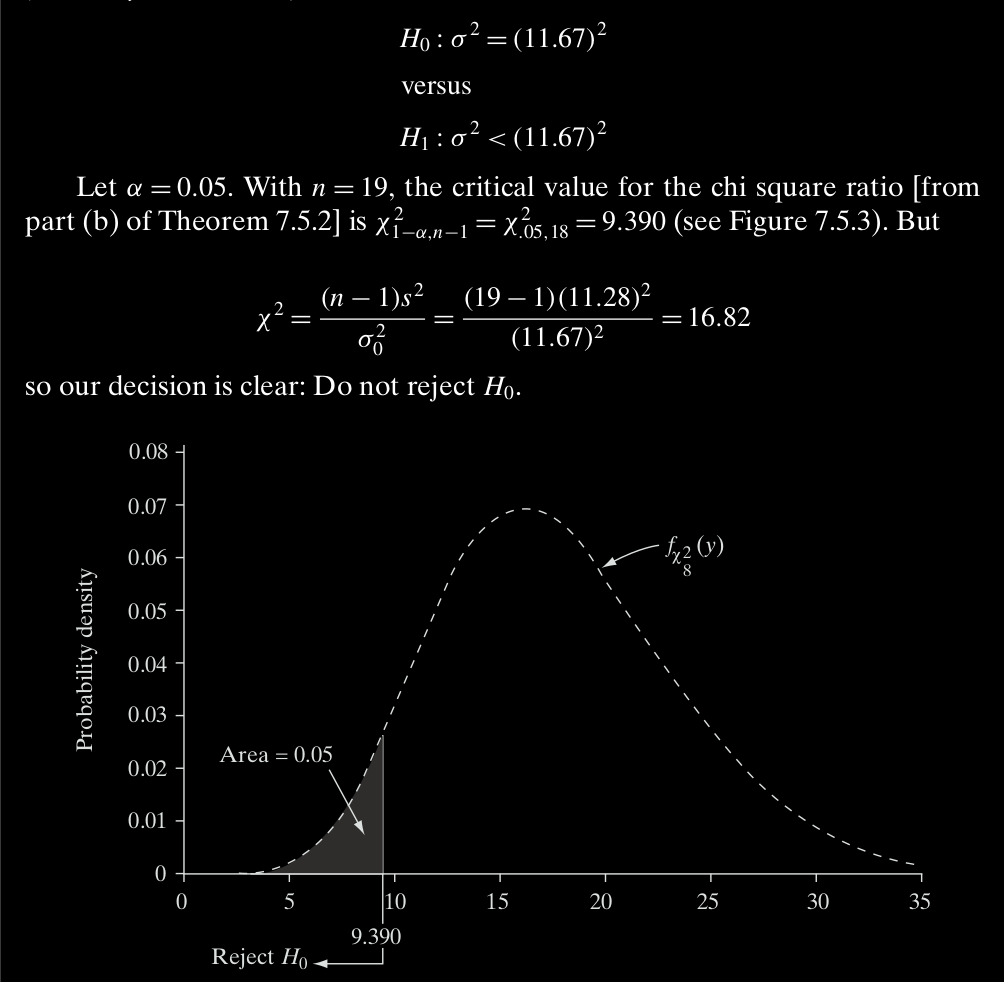
\includegraphics[scale=0.25]{Case_7-5-2-2-neg.png}
\end{frame}
%-------------- end slide -------------------------------%}}}

\end{document}


